\documentclass[12pt]{book}

\usepackage[T1]{fontenc}
\usepackage[utf8]{inputenc}
\usepackage[english]{babel}
\usepackage{graphicx}
\usepackage{tabulary}
\usepackage{mathtools}
\usepackage{amsfonts}
\usepackage[autostyle]{csquotes}

\usepackage{textcomp}                   % For the special character ° and TM

\usepackage{cranfieldthesis}            % Use the custom "cranfieldthesis" LaTeX style file. 

\usepackage[sorting=none, backend=biber, style=numeric]{biblatex}
\usepackage[colorlinks=false]{hyperref}

\usepackage{tikz}
\usetikzlibrary{shapes, arrows, trees, calc}

% By default, LaTeX uses a serif font - these are traditionally thought to be
% easier to read.   If you'd prefer sans-serif, please uncomment the 
% following line.
%\renewcommand{\familydefault}{\sfdefault}

\newcommand{\TM}{\textsuperscript{TM}~}
% \newcommand{\source}[1]{\caption*{\hfill Source: {#1}} }

% Example parameters for a typical taught MSc course
\title{Automated food log analysis}
\author{NOGARET Baptiste}
\date{\today}
\school{Aerospace, Transport and Manufacturing}
\course{Computational and Software Techniques in Engineering}
\degree{Master of Science}
\academicyear{2015--2016}
\supervisor{Dr RÜGER Stefan}
\copyrightyear{2016}

\addbibresource{library.bib}
\addbibresource{my_references.bib}

\newcommand{\E}{\mathbb{E}}
\newcommand{\N}{\mathbb{N}}
\newcommand{\Var}{\operatorname{Var}}
\newcommand{\argmin}{\operatorname {arg\,min} }
\newcommand{\argmax}{\operatorname {arg\,max} }
\newcommand{\sign}{\operatorname {sign} }

\begin{document}


% Front matter
\frontmatter

% Standard-Form Title Pages
\maketitle

% Declaration of authorship
\chapter{Declaration of authorship}



% Abstract and Keywords
\begin{abstract}
    
    Automated food log is a promising exemplar of image analysis which allow users to keep pictures that are processed to keep track automatically of one's food intake. It is a challenging problem due to the high variability of dishes (picture conditions, various types, plating).
    
    With this purpose, the presented master thesis describe a process for simultaneous localisation and recognition. To tackle this problem, several feature descriptors and classifiers were sought to obtain the highest efficiency. From the experiments, the leading method is based on two steps, with first a convolutional neural network pre-trained to detect salient objects is applied on each image to generate bounding boxes for each food area and second, an additional convolutional neural network is used in combination of random forest to recognize the food in each bounding box.
    
    Evaluated on the UEC-FOOD 256 dataset, the method enhances the current best segmentation algorithm with 74\% of top-1 accuracy. Overall, an accuracy of 28 \% were obtained.
    
    \section*{Keywords}
    Food log; Photo; Localisation; Classification; Convolutional neural network
\end{abstract}

% Table of Contents
\sstableofcontents

% List of Figures
\sslistoffigures

% List of Tables
\sslistoftables

% The list of abbreviations can't be automatically generated so you need to populate it yourself
\begin{listofabbreviations}
    \abbrev{CNN}{Convolutional Neural Network}
    \abbrev{LBP}{Local Binary Pattern}
    \abbrev{SIFT}{Scale-Invariant Feature Transform}
    \abbrev{SURF}{Speeded Up Robust Features}
    \abbrev{SVM}{Support Vector Machine}
\end{listofabbreviations}

% Acknowledgements
\chapter{Acknowledgements}

I am really grateful to Dr. Stefan Rüger, my supervisor for the project, to have proposed this subject. His guidance and valuable advice were particularly helpful to realise the thesis.

Moreover, I would like to thank the University of Technology of Compiègne for giving me the opportunity to study one year in Cranfield University. I would also like to thank Cranfield University for its facilities.

I would like to express my gratitude to M. Kazu Shimoda and Pr. Keiji Yanai of the University of Tokyo that provided enlightenments and further details on their work and datasets.

%% Main Matter
%
% This is where we include the main thesis content.
%
\mainmatter

\chapter{Introduction}

Over the last few decades, the rate of obesity and overweight people in the World has greatly increased. As presented for the UK case in the Fig. \ref{fig:obesity_uk}, the obesity rate has increased by 12\% between 1980 and 2013, and the overweight rate by 13\%. It is forecast by the World Health Organisation to continue to grow in the next decades.

\begin{figure}[h]
    \centering
    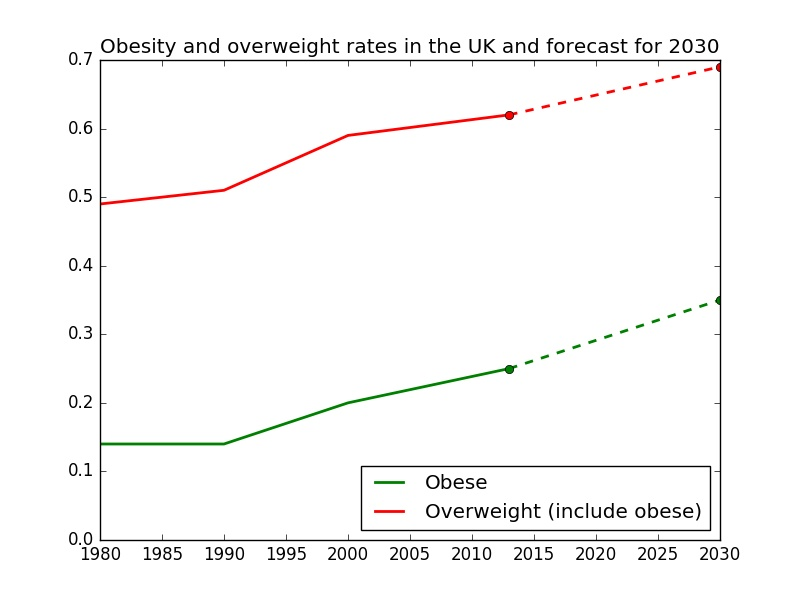
\includegraphics[width=0.5\textwidth,  height=0.455\textwidth ]{img/obesity_uk.jpg}
    \caption[Obesity and overweight rate of the adult population in the uk between 1980 and 2030. \textit{Source: World Health Organisation}]{Obesity and overweight rate of the adult population in the uk between 1980 and 2030}
    \label{fig:obesity_uk}
\end{figure}

Being \enquote{overweight} is defined as having a Body Mass Index (BMI) – a person's weight in kilograms divided by the square of his height in meters ($ kg / m^2 $) – of between 25 and 29.9, and \enquote{obese} by a BMI of 30 and above.

As stated in \cite{Mokdad2003}, obesity is strongly associated with several major health risk factors such as stroke, high blood pressure, type 2 diabetes and high cholesterol. Thus, it has a great human and economic (Zhang et al. \cite{Zhang2010} in 2010 showed 12\% of the total worldwide health expenditure is spent on diabetes and the total cost will continue to grow) cost for societies.

Associated with lifestyle changes, recording what we eat is one way to control our eating. Studies such as \cite{Burke2011a} show the benefit of reporting its daily diet to lose weight and improve the quality of its food intake. And more generally, it can be a way to treat eat disorders

Yet, manually recording detailed information regarding all meals is a tedious and time consuming task and it is hard for people to adhere to this process for a long time. Moreover, it often needs a trained patient. As presented in \cite{Lichtman1992}, user logs are prone to errors (users tend to underestimate its intake).

At the same time, image processing methods has greatly improved the recognition rate of elements in a picture. ImageNet is a dataset containing more than 1,2 million images split into 1000 classes. Since 2010, the yearly challenges include localisation, classification and detection. Numerous researchers, students, educators or information technology companies are participated.

As described in Fig. \ref{fig:imagenet_results} and using data from the challenge result report \cite{Russakovsky2015}, the mean classification error for each class and localisation has been greatly reduced between 2010 and 2014.

\begin{figure}[h]
    \centering
    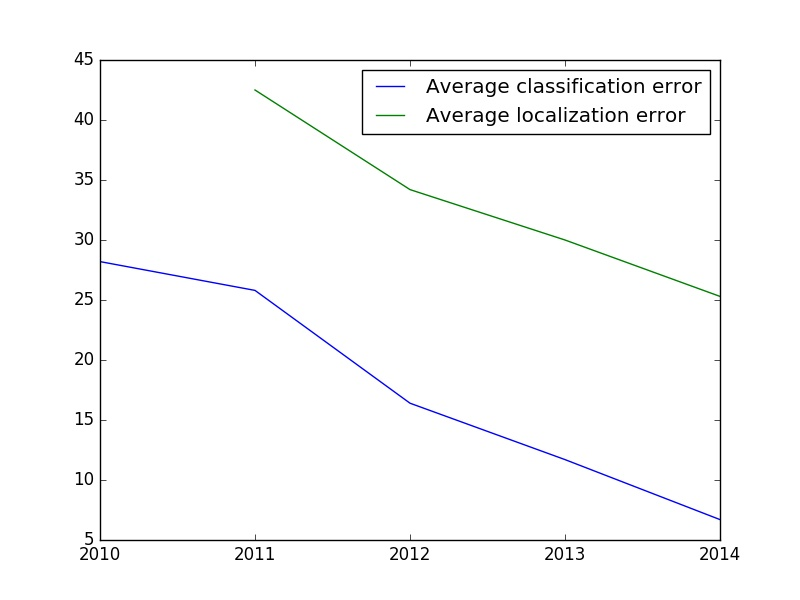
\includegraphics[width=0.5\textwidth,  height=0.455\textwidth ]{img/imagenet}
    \caption{Average classification and localisation error of the best results for different ImageNet challenges}
    \label{fig:imagenet_results}
\end{figure}

With the widespread use of smartphone, cameras or wearable devices, people can easily take pictures of a good quality and are already taking photos of their food and posting them on website such as Food Gawker, Instagram, Flickr or Yelp.

That's why, it has recently been proposed to automate the process and assist patient and their medical personnel (nutritionists, psychologists) to understand the patient's behaviour and habits. It extends the reach of care in a cost effective ways and counters some of the previous problem of manual report. It's part of the rise of e-healthcare / m-healthcare \cite{Hillestad2005, Menachemi2011}.

The idea is to have users who upload pictures of their daily meals to the application or website that constructs their food diary automatically. Using image processing, it estimates the dietary composition of the meal and keep record of the information for later viewing in formats such as tables or graphical representations.

Food recognition is a promising applications of image processing and machine learning. Its overall process is:
\begin{itemize}
    \item Extract key characteristics
    \item Localise food items if the application allow multiple food items
    \item Recognise the food
\end{itemize}

Feature description is essential to achieve good object detection and image categorisation. Preferably the method should be invariant of the conditions, i.e. the luminosity, orientation or scale of the picture.

In this thesis, we focus on the food recognition. It has already numerous challenges such as:
\begin{itemize}
    \item \textbf{high intra-class variability} : we can have high variability between pictures for the same particular kind of food items, due to:
    \begin{itemize}
        \item environmental conditions (e.g. luminosity, quality of the camera)
        \item plating (the way it is served)
        \item variation of the way the picture is taken: numerous transformation can be applied to a same picture (scale, translation, rotation, skewness, crop)
    \end{itemize}
    This is illustrated in Fig. \ref{fig:intra-class_variability} for pictures of kaya toast.
    
    \item \textbf{low inter-class variability} : we can have low variability between different type of food such as between clear and miso soup as showed in Fig. \ref{fig:inter-class_variability}.
\end{itemize}

This makes localisation, classification and retrieval of food images a difficult task for current state-of-the-art techniques, and hence a compelling challenge for image processing and machine learning researchers.

Thus, the thesis is dedicated to the investigation on some methods that were found in the literature. Many modi operandi exist and we focus on three different descriptors: colour and texture features, local feature using Bag-Of-Word representation and convolutional neural network. These methods are evaluated on UEC-FOOD 256 and compared to previous papers. The generation of this dataset was presented by \cite{Kawano2015} by Kawano et al. from the University of Tokyo in 2015.

\begin{figure}
    \centering
    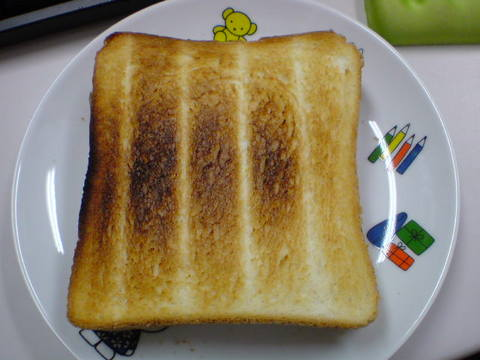
\includegraphics[height=4cm, width=4cm]{img/kaya_toast_1.jpg}
    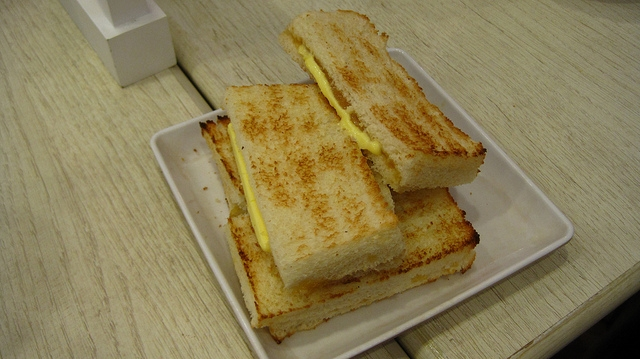
\includegraphics[height=4cm, width=4cm]{img/kaya_toast_2.jpg}
    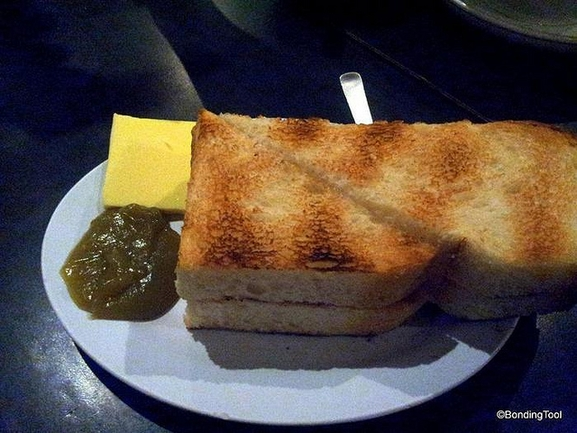
\includegraphics[height=4cm, width=4cm]{img/kaya_toast_3.jpg}
    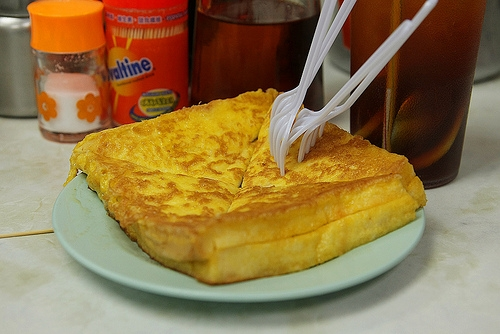
\includegraphics[height=4cm, width=4cm]{img/kaya_toast_4.jpg}
    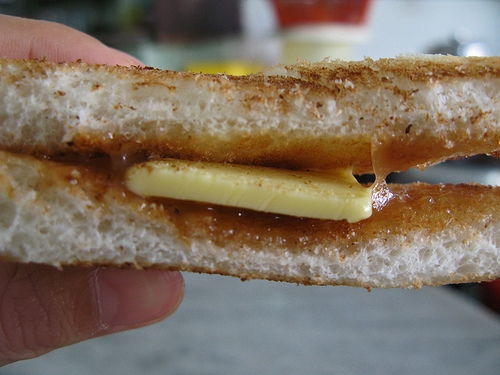
\includegraphics[height=4cm, width=4cm]{img/kaya_toast_5.jpg}
    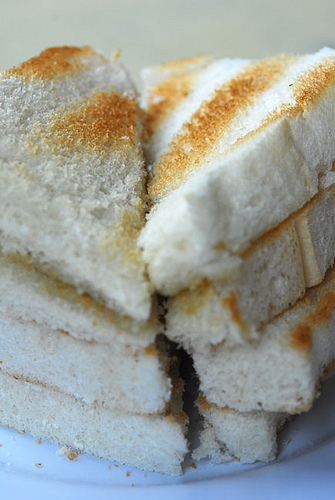
\includegraphics[height=4cm, width=4cm]{img/kaya_toast_6.jpg}
    \caption[Examples of high intra-class variability for kaya toast]{Examples of high intra-class variability for kaya toast. Pictures extracted from the UEC FOOD 256 dataset \cite{Kawano2015}.}
    \label{fig:intra-class_variability}
\end{figure}

\begin{figure}
    \centering
    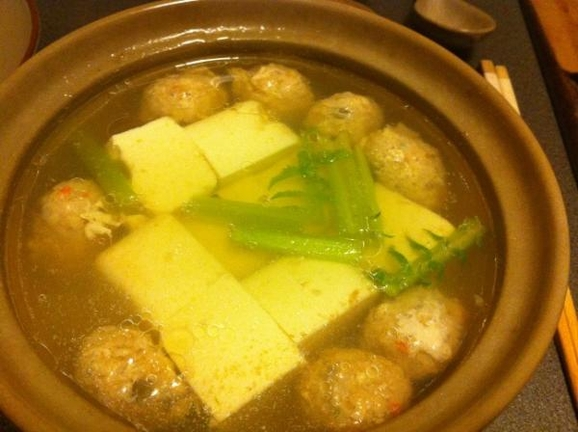
\includegraphics[width=7cm, height=6cm]{img/clear_soup.jpg}
    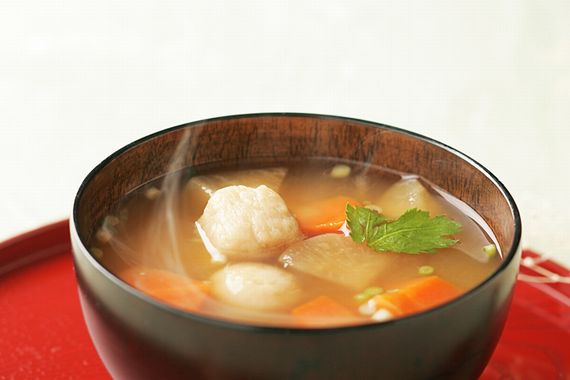
\includegraphics[width=7cm, height=6cm]{img/miso_soup.jpg}
    \caption[Examples of low inter-class variability for kaya toast]{Examples of low inter-class variability for clear soup (left) and miso soup (right). Pictures extracted from the UEC FOOD 256 dataset \cite{Kawano2015}.}
    \label{fig:inter-class_variability}
\end{figure}

The organization of this thesis is as follow. In section \ref{sec:previous_work}, previous work on food localisation, recognition and intake estimation is reviewed. Section \ref{sec:feature_descriptor} introduces the different image descriptors used, and in section \ref{sec:classifier} the classifiers are presented. In section \ref{sec:dataset}, the dataset is introduced. Section \ref{sec:evaluation} reports the experimental settings and results. Finally, in section \ref{sec:conclusion}, we draw the conclusion and state the limitation and possible future work.


\chapter{Previous work} \label{sec:previous_work}

A profusion of techniques have been employed in the literature for food recognition. Yet, localisation and classification have been rarely used simultaneous. That is why these two subjects are presented separately (section 2.1 is dedicated to food localisation, section 2.2 to recognition). Then, some food applications are presented.

\section{Food localisation}

%% Color and edge segmentation
%% 11.1

A way to localize food is based on edge detection and colour segmentation.

In \cite{Thendral2014a}, Thendral et al. describes and compare these two methods to localise an orange in a picture. It applied these methods on a small dataset of 20 orange images (only one orange per image), with different lighting conditions and backgrounds (pictures are taken from the Internet).
In more details, the edge-based segmentation apply the canny-edge segmentation, then apply non-maximum suppression to eliminate noises. Then, each pixels are classified.
The colour-based segmentation normalised the lightning condition with a Gaussian low-pass filter, convert the RGB image into a $L * a * b$
\begin{enumerate}
    \item Gaussian low pass filter to normalize the lightning condition
    \item convert the image from RGB representation to $L * a * b$
    \item use the $a$ channel to classify each pixel as \enquote{fruit} or \enquote{non-fruit}
    \item remove small object
    \item fill the binary image regions and holes
\end{enumerate}
For orange detection, the colour segmentation has an higher accuracy. Yet, it is very hard to generalise this method as it has only been tested on oranges, a food item with a very distinctive colour.

%% Circle
%% 2.2 (partial) + 6.3 + \cite{Dehais2015} ?

An other method for food detection relies on circle detection. Indeed, food items are often served in a round shape container such as a bowl, pan or plate.

In \cite{Wazumi2011}, Wazumi et al. describe their use of the Hough transformation. The purpose of this technique is to find approximations of instances a certain class of shapes by a voting procedure. In this paper it is used to detect circles assuming the food is only contained in round plates or bowls and with edges not obstructed on the picture (it performs poorly with cropped pictures). Keeping only the central part of the circle, the segmentation is then fed to the recognition process.

%% CNN
%% DCNN: * ? + 9.1 (in food intake)
%% Presentation of UEC FOOD 100 and 256

A more recent development is the used of convolutional neural network.

In \cite{Shimoda2015}, Shimoda et al. presents their segmentation process based on a pre-trained deep CNN.

The proposed pipeline is composed of 6 main steps:
\begin{enumerate}
    \item detect all the possible bounding box (maximum 2000 per image) using selective search
    \item cluster the bounding box, using the ration of intersection over union (IOU, also call overlap ratio) to obtain 20 at most.
    \item a Deep CNN for all the selected bounding box to get a saliency map. The DCNN is modelled on AlexNet CNN, was pre-trained on the Salient Object Subitizing (14 000 everyday pictures) dataset and fine-tuned on UEC FOOD 100.
    \item use the GrabCut algorithm to extract the foreground region from the food area. GrabCut is an iterative method using graph cuts to extract foreground from background based on an initial guess.
    \item In case of overlapped bounding box, the authors proposed to apply the non-maximum suppression (NMS) algorithm.
\end{enumerate}

The authors apply this process on the UEC-FOOD 100 dataset and PASCAL VOC 2007. The latter is used for object detection and recognition of 20 common classes (train, tv, cat, human ...)). These two datasets use bounding box to spot items. A segmentation is correct if the overlap ratio exceeds 50\% between the predicted and the ground truth bounding box.

UEC FOOD 100 \footnote{Dataset can be found at \url{http://foodcam.mobi/dataset100.html}} is a dataset created by Matsuda et al. in \cite{Matsuda2012a} containing 100 types of food, mainly Japanese food, and is composed of 9060 pictures. Thus, an image can contain multiple dishes. That's why each food picture is associated with the bounding box coordinates indicating the food localisation.

For UEC-FOOD 100, the authors obtain 49.9\% mean average accuracy and 58.7\% for PASCAL VOC 2007.

A pre-trained DCNN is also used by Bolanos et al. \cite{Bolanos2016} to classify each pixel as food or non-food. The DCNN is modelled on \enquote{GoogleNet} \cite{Szegedy2015}, a neural network composed of 22 layers and first used on ILSVRC14 (ImageNet Large Scale Visual Recognition Competition 2014). On UEC-FOOD 256, the authors obtain 60\% of accuracy.

UEC FOOD 256 \footnote{Dataset can be found at \url{http://foodcam.mobi/dataset256.html}} is presented in \cite{Kawano2015} and it is an extension of UEC-FOOD 100 (same creators' team). It adds 156 kinds of food from all the over the world (French, Italian, Vietnamese, American, ...). As for UEC-FOOD 100, every food photo has a bounding box indicating the food location.

\section{Food recognition}

Over the last few years, authors have focused on food recognition. Various methods were tried. For feature extraction, it often combines colour and texture descriptors, global and local.

In \cite{Chen2009}, Chen et al. create a new dataset named PFID and provide two simple food classification baseline methods. PFID (stands for Pittsburgh fast-food image dataset) \footnote{Dataset can be found at \url{http://pfid.rit.albany.edu/}} was presented in \cite{Chen2009} in summer 2008 from the collaboration of Intel Labs Pittsburgh, Columbia and Carnegie Mellon universities. It is one of the first mature datasets released for food recognition.

It contains 101 meals (categories) from 11 popular fast food chains found in the USA with images and videos captured in both restaurant conditions and controlled lab setting. It contains foods such as chickens, sandwiches, salads, burgers and drinks from Arby's, Bruggers Bagels, Dunkin Donuts, KFC, McDonalds, Panera, Pizza hut, Quiznos, Subway, Taco Bell and Wendy's.

In their paper, Chen et al. provide two baseline methods:
\begin{itemize}
    \item Colour histogram and SVM classifier. They obtain a mean accuracy of around 12\%.
    \item Bag-of-Features using SIFT and SVM classifier. They obtain a mean accuracy of around 25\%.
\end{itemize}

Song et al. \cite{Zong2010} use also a Bag-of-Word method using SIFT for detection of the keypoints and LBP for description. They use a local texture feature and their spatial distribution to classify food images from the PFID. The shape context algorithm is used to keep the spatial relationship between codewords (for each image, compute the histogram of one word compared to the others / then mean of the histograms).

For the classification, the authors pick the smallest cost between an image and a food category. For each interest points found with SIFT in the image, we associate a similarity between the point and each visual words of the codebook. The similarity function is based on the Bhattacharyya distance. Then, the shape context between the point of interests and the visual word is calculated and a cost is deduced for each food category. The category with the smallest cost is chosen.

Regrouping the different pictures in 6 main groups the PFI dataset (sandwiches and wraps, meat, salads, donuts, hamburger and miscellaneous), they obtain an average accuracy of 66\%.

Moreover, Fast foods, as they are standardized and have nutrition information available online, can easily be used to measure the calories. In \cite{Wen2009}, the authors are using the PFID's videos to estimate energy intake of a meal.

While Chen et al. use global and local features separately, Bosch et al. \cite{Bosch2011} combine to identify the food consumed. For the global features, they use colour properties (entropy, histogram and moments) with texture information provided by Gabor filters. They add local features with the Bag-Of-Features, using SIFT for detection and SIFT, steerable filters and DAISY descriptors. To classify, they use SVM (using the Radial Basis function kernel). On a in-house dataset composed of 28 classes and 179 images, the authors obtain 86\% of accuracy.

% 4.3 (PFID)

Still evaluated on PFID, Yang et al. \cite{Yang2010} use a novel feature, named PFD (for pairwise local feature distribution) for food recognition.

The different steps of this method are:
\begin{enumerate}
    \item classify each pixel in one of the categories between beef, chicken, pork, bread, vegetable,  tomato/tomato sauce, cheese/butter, egg/other and background. For classification, they use the Semantic Texton Forest, method based on local characteristics. It was previously trained on 16 manually-labelled pictures.
    
    \item Global ingredient representation (GIR): for the 8 food categories, it sum up the soft label of all the ingredient pixel and normalize by the number.
    
    \item PFD: geometric pairwise feature on N ingredient pixels (picked randomly, thus N / 2 pairs):
    \begin{itemize}
        \item log of the distance
        \item orientation
        \item soft label of the midpoint
        \item soft label of each pixel along the line connecting the pair of pixels
        \item joint feature (a mixed of the above characteristics)
    \end{itemize}
    Accumulate the pairwise values into a distribution (using a multi-dimensional histogram of either 8 or 12 bins), weighted by the soft labels of the two pixels. Each pixel is mapped to its closest bin in the histogram.
    Then, normalization of the histogram.
\end{enumerate}

Fed to a linear SVM, they obtain an accuracy between 19\% and 28\% for each of the 61 categories.
When they pick the 6 major types of food, they get almost 80\% of accuracy.

% ETHZ Food 101
% 2.1

In \cite{Bossard2014}, the author use the Random forest clustering algorithm to create superpixels (selecting only the discriminative one). On these superpixels, a dense SURF and L*a*b* color value is computed and encoded with improved fisher vectors (IFV) with Gaussian mixture model (GMM) of 64 Gaussians.
Then, they use PCA to reduce the size of the vector and the machine learning method is structured-output multi-class SVM. They use their method on their new dataset named ETHZ Food-101 (56\% accuracy) and MIT-indoor (58\% of accuracy on the full dataset) and compare it against several previous implementations.

ETHZ Food-101 \footnote{Dataset can be found at  \url{https://www.vision.ee.ethz.ch/datasets_extra/food-101/}} is composed of 101 categories, 1000 images per category (250 pictures manually reviewed, used for the test set and 750 with noises for the training test). Pictures were extracted from the website \href{http://www.foodspotting.com/}{foodspotting.com}. The top 101 most popular dishes from this social sharing food images defined the categories.

% 8.3

\cite{Chen2012} present a method to automatically identify food and estimate the quantity. It is used on an in-house dataset composed of 50 categories, mainly Chinese fishes, with 100 pictures per class. For recognition, the authors use:
\begin{itemize}
    \item local information with Bag-Of-Words, using SIFT as descriptor and Local binary pattern on a 3-level pyramid
    \item global information: colour histograms and Gabor filters extracted from of each block (image divided into $4 \times 4$ blocks)
\end{itemize}

They train a SVM classifier for each category, then fuse them with the multi-class AdaBoost algorithm. AdaBoost, or \enquote{Adaptive boosting} is a meta-algorithm that combine into a weighted sum multiple classifiers to improve their final performance.
The authors get an overall accuracy of 68.3\%. If we keep the top-3 results, the accuracy is even 90.9\%.


%% DCNN

More recently, people have started to heavily use Convolutional Neural Networks \textit{CNN} with great results.

%% UMPC Food 101
%% 8.1

In \cite{Wang2015}, the authors created a new dataset named UMPC Food-101 ("twin dataset" of ETHZ Food 101) combining text and visual information for recipes. As a proof of concept, they develop a search application for recipe recognition. The user send a query (a food image) and as a result, the three best recipes (categories) are displayed.

UMPC Food-101 \footnote{Dataset can be found at \url{http://visiir.lip6.fr/}} is a \enquote{twin-dataset} of ETHZ Food 101 as it is composed of the same 101 categories, with 1000 images per category. Yet, the pictures have been crawled from Google image, researching for recipes. Thus, most images are associated with a text.

For the image recognition model, they use textual, visual or a mix of both features:
\begin{itemize}
    \item visual feature (all feeding a SVM):
    \begin{itemize}
        \item Bag-of-Words using a dense SIFT and a codebook of size 1024 on a 3-level spatial pyramid. They obtain an average accuracy of 23.96\%.
        
        \item Use an improved version of the Bag-of-Words named \enquote{BossaNova}. It modifies the pooling system; instead of keeping the closest cluster of a SIFT descriptor, it represents it by keeping distances between the descriptor and all the codebook words. Average accuracy of 28.59\%.
        
        \item Use a deep CNN as a feature descriptor, using the 7th layer of a pre-trained CNN ("OverFeat"). Average accuracy of 33.91\%.
        
        \item Use a very deep CNN as a feature descriptor, using th 19th layers ("vgg-verydeep-19"). Average accuracy of 40.21\%.
    \end{itemize}
    
    \item text-feature: use the term frequency - inverse document frequency \textit{tf-idf} method and get 82.06\% accuracy
    
    \item fusion of textual and visual feature: they obtain at most 85.10\% of accuracy, combining the very deep CNN descriptors and tf-idf.
\end{itemize}

%% UEC FOOD
%% 2.3

In \cite{Kawano2014}, the authors use a pre-trained Deep CNN \textit{DCNN} for feature extraction. The DCNN, called \enquote{OverFeat}, \footnote{Can be found \url{http://cilvr.nyu.edu/doku.php?id=code:start}} was trained on ImageNet and is composed of 19 layers. The authors add more conventional image features to obtain feature vectors composed of: 
\begin{enumerate}
    \item a variant of the Histogram of Oriented Gradients \textit{HOG} called \enquote{Root Hog} that is an element-wise square root of the L1 normalized HOG
    \item mean and variance values of each channel of the RGB representation value of pixels from each of 2*2  block
    \item the last two layers of the DCNN
\end{enumerate}
The three descriptors are then encoded in a fisher vector. Using SVM, the authors obtain 72\% of  accuracy for UEC-FOOD 100.

%% UEC FOOD 256

In \cite{Yanai2015}, the authors use a fine-tuned pre-trained DCNN with the large-scale ImageNet dataset for food recognition. The authors obtain 79\% average accuracy for UEC FOOD 100 and 67\% for UEC FOOD-256.

In \cite{Bolanos2016}, the authors also use a fine-tuned pre-trained Deep Neural Network and obtain 63\% accuracy on UEC FOOD-256. Their neural network is fine-tuned on multiple food datasets (UEC FOOD 256, Food 101 and EgocentricFood).

\section{Food log application and intake estimation}

%% Food Log

FoodLog \footnote{\url{http://www.foodlog.jp}} is a website that enables the user to upload pictures of its daily meals to be archived and processed. The goal of this application is to assist the user to keep notes of their meals and balance the nutritional values coming from different kinds of food.

In \cite{Kitamura2008}, the images containing food items are identified by exploiting features related to the HSV and RGB colour domains, as well as the shape of the plate. A SVM classifier is trained to detect food images. More specifically, the images are divided in 300 blocks and each block is classified as \enquote{non-food} (discarded block) or one of the nutritional categories described in the \enquote{MyPyramid} model \footnote{\url{http://www.mypyramid.gov}}.

MyPyramid \cite{MyPyramid} was designed by the United State Department of Agriculture \textit{USDA} in 2005 and was replaced in 2011 by \enquote{MyPlate} \footnote{\url{http://www.choosemyplate.gov}} \cite{MyPlate}. This dietary model is composed of 5 kinds of food: grains, vegetable, meals and beans, milk and fruit. For each group, a recommended intake per day is associated, Fig. \ref{fig:my_pyramid}. Quantity is categorized by \enquote{servings} \textit{SV}, making it simpler to compute and keep log.

\begin{figure}
    \centering
    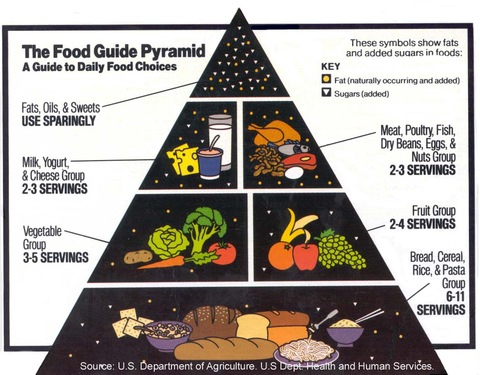
\includegraphics[scale=0.7]{img/my_pyramid.jpg}
    \caption[USDA MyPyramid original logo]{USDA MyPyramid original logo. Source \href{https://en.wikipedia.org/wiki/Food_pyramid_(nutrition)}{Wikipedia}.}
    \label{fig:my_pyramid}
\end{figure}

In \cite{Aizawa2013} the Support Vector Machine is replaced by a Bayesian Framework \textit{BF} to improve the classification, taking into account the previous picture of a specific user to update the classifier. The BF is based on the Gaussian Naive Bayesian (suppose independence between every pair of features and the distribution of each feature is assumed to be Gaussian). The BF takes into account the estimation using colour moments and Bag-Of-Feature of SIFT, the prior distribution and the mealtime category (breakfast, lunch and dinner). 
The team further improve their accuracy in \cite{Kagaya2014}. Kagaya et al. use a Convolutional Neural Network \textins{CNN} to detect and classify food from a small subset of image loaded in the FoodLog system. Compared to the other conventional methods (use of a feature descriptor such as Bag-of-Words with a classifier, e.g. SVM) described previously, the CNN showed a significantly higher accuracy.

%% Others

An other method to estimate the food intake is to evaluate the food volume.

In \cite{Chen2012}, the authors presents a method that use the depth information of the picture. Once the food has been classified, the area of the food container (bowl, plate) and the depth value of the contained food is computed to obtain the food volume.
Yet, this technique is still limited as it can only be used for non-transparent food, i.e it can't detect some food item such as water or cooked rice, and force the user to have a depth camera (such as Kinect).

Without depth information, the volume can also be estimated as in \cite{Almaghrabi2012a}. Almaghrabi et al. presents a novel food recognition system that is able to estimate of the nutrition intake. Moreover, they develop a mobile application to easily take pictures and keep track of the user's diet. To measure the food intake, authors compare before and after eating pictures and use the thumb as the calibration system (it supposes a one-time calibration to know the size of the thumb of the user).
The process to show the intake is:
\begin{enumerate}
    \item the user takes food pictures
    \item get the contour of each picture
    \item recognition of the food using colour, shape and size features with SVM.
    \item volume calculation, that is computed in two steps:
    \begin{enumerate}
        \item user takes a picture from above. Then, the food shape is divided into known shape (rectangle, circle, triangle ...) to compute the area.
        \item user takes a second picture from the side. This is used to compute the height of the food and calculate the overall volume.
    \end{enumerate}
    The system assumes that the plate is white and round.
    \item use a nutrition database to obtain the average calories
\end{enumerate}
If the user has not eaten everything, the entire must be repeated.
The drawbacks of this method is the user have to take several pictures, with one's thumb each time and it has been tested with a limited set of simple food types.

%
% Zhu
%

In \cite{Zhu2010}, the authors develop a mobile application to keep food records of a user that is taking pictures of one's meal. Their method can detect multiple food items in one picture. They use a colour marker (color chequerboard) as an illumination and size indicator.
As in \cite{Almaghrabi2012a}, images obtained before and after foods are eaten are used to estimate the amount of food consumed.

When the user upload a picture, it is segmented, then classified by a back-end server. The estimation (labelled image with food type and volume) are sent back to the user for confirmation.

For segmentation, the authors use connected component analysis, active contours, and normalized cuts. Then, colour and texture features are extracted to feed a SVM classifier. The authors use:
\begin{itemize}
    \item Gabor filters. Gabor filters describe properties related to the local power spectrum of a signal and have been used for texture analysis
    \item 2-D colour histograms of the a* and b* channels of the CIELaB representation. Values are corrected using the colour marker
\end{itemize}
For the volume estimation, the authors use a 3-D volume reconstruction process. The food area is partitioned and assigned to \enquote{geometric classes}, each with their own sets of parameters.

They evaluate their segmentation and classification methods on a very small dataset composed of 63 images and 19 classes. The authors obtain an average accuracy of 89\%.

In \cite{Zhu2015}, their method is named \enquote{multiple hypotheses segmentation and classification} \textit{MHSC}. It is an iterative algorithm composed of a segmentation, description (extraction of features) and classification steps.

For segmentation, the authors first detect salient region, using Canny edge and colour distribution to reject background. Then, they apply a multi-scale segmentation using normalized cut. Small segmented regions are discarded.

On the selected region, the authors used a mixed of global descriptors (first and second moment of each channel for RGB, YCbCr, L*a*b*, and HSV colour spaces, first and second moment of the entropy in RGB, predominant colour descriptor, entropy and two first moments of the Gradient Orientation Spatial-Dependence Matrix, entropy categorization and fractal dimension estimation and estimation of the fractal dimension of the response of different Gabor filter) with local feature (multi Bag-Of-Words using SIFT for RGB, SURF for RGB, SIFT for each channel of the RGB representation and steerable filters).

Each of the 12 descriptor, global and local, is classified independently and assigned a confidence score. A late fusion function (either maximum confidence score or majority vote) is used  to decide the final class. For classification, the authors use K-NN and SVM.

If the total score is inferior to a certain threshold, the overall process is repeated. The confidence score of the previous step is used to improve the segmentation.

Applied on a dataset composed of 83 labels (79 food classes plus \enquote{utensils}, \enquote{glasses}, \enquote{plates}, and \enquote{plastic cups} classes), each class having at least 30 images, they obtain a top-8 accuracy of 75\%, using K-NN with the maximum confidence score.

%% Food Cam
%% 6.3

In \cite{Matsuda2012a}, the authors propose a food recognition system named \textbf{FoodCam} to identify food items of a picture. The presented process is used on a mobile application, the user taking a picture that is transferred to a sever, processed and results are displayed.

The first step is to detect potential region with multiple object detection algorithms. Then, for these regions, several feeatures are extracted and used to feed SVM with Multiple Kernel Learning \textit{MKL} method. To detect candidate regions, the authors use:
\begin{itemize}
    \item Felzenszwalb’s deformable part model (DPM), based on Histogram of Oriented Gradients (HOG).
    \item a circle detector: the image is converted to a gray-scale, contour are extracted using the Canny Edge Detector and circles detected by the Hough Transform
    \item JSEG region segmentation: segment region based on colour. It only keeps circular regions.
    \item whole image, for picture with one large dish
\end{itemize}
Then, it aggregates all the candidate regions to get the bounding box of each food item.

For each region, it extracts multiple common features:
\begin{itemize}
    \item Bag of Feature of SIFT and C-SIFT (sift with colour invariant characteristics)
    \item Spatial pyramid representation: object regions are divided by hierarchical grids. In this paper, the three level pyramid is used: $1 \times 1$, $2 \times 2$, $3 \times 3$. For each grid, a BoF vector is extracted
    \item Histogram of Oriented Gradient (HOG)
    \item Gabor texture
\end{itemize}

After extraction of the feature vectors from each candidate region, a linear SVM trained by MKL is used ($\chi^2$ kernel). Their methods were evaluated on UEC-FOOD 100. For multiple food item images, they obtain 55.8\% classification rate and 68.9\% for single food item pictures.

%% 

In \cite{Kawano2014a}, the authors develop a mobile real-time food recognition system for calorie and nutrition estimation. Contrary to the previous paper, all the calculation are realised on the user smartphone. The recognition takes less than 1 second thanks to the multi-core architecture of modern smartphones.
The user takes a picture and draws bounding boxes around food items. Then, the system refine the segmentation based on the users' rough demarcation using Grabcut.
For each item, it extracts image features and classify the image among the one hundred food classes using a linear SVM. Then, the top five food candidates are shown and the user can select one of the proposition.
This recognition is updated every one second, the direction arrow as presented in Fig. \ref{fig:food_cam} being displayed to help the user improve the result by changing the camera position and direction. To estimate the most suitable direction, the authors use the Efficient Sub-window Search method, a recent and powerful window search algorithm used in object detection.
The mobile application keep records of all the pictures and their approved classification and labelled with the volume estimation. Food intake is estimated thanks to a slider on the bottom-left of the screen.

\begin{figure}
    \centering
    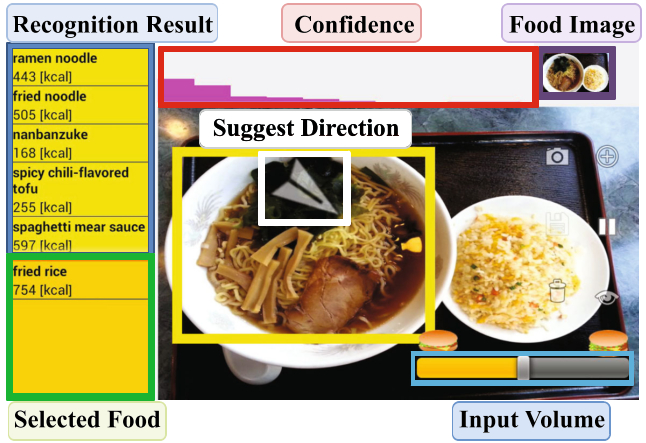
\includegraphics[scale=0.6]{img/foodcam.jpg}
    \caption[Annotated screenshot of the FoodCam application]{Annotated screenshot of the FoodCam application. Source \cite{Kawano2014a}.}
    \label{fig:food_cam}
\end{figure}

Two different descriptors are used:
\begin{itemize}
    \item bag-of-feature, SURF for detection and description, and colour histogram with the $chi^2$ kernel feature map
    \item HOG and a colour patch descriptor (mean and variance of RGB values on a $2 \times 2$ blocks of pixel) encoded using Fisher Victor, a patch encoding strategy using Gaussian mixture models.
\end{itemize}
The authors evaluate these two methods on UEC-FOOD 100. Taking the top 5 classes, they obtain 79\% classification accuracy for colour patches and 68\% for the other.

%% 11.2

In \cite{Bettadapura2015}, the authors develop an application to recognize food items from an image taken by the user in a restaurant. It uses some contextual data (the geolocalisation) to improve the classification. Indeed, they use geolocalisation to get the menu from internet and query Google Search to get images (extract the top 50 pictures) of 15 dishes from the menu. These images are used as weakly-labelled training pictures to improve the recognition accuracy.

The first step is the segmentation to localize the food and ignore the background through hierarchical segmentation. Then, colour moment invariants, hue histograms, Bag of Words of SIFT, RGB SIFT (SIFT component for each RGB channel), C-SIFT (a color invariant SIFT), Opponent-SIFT (SIFT on colour-opponent channels) are used as feature descriptors. For the 4 SIFT representations: they build a codebooks of 100 000 visual words (using k-means clustering, k = 1000) to build Bag-of-Word histogram.

Then, for the image classification, they adopt the SMO-MKL (Sequential minimal optimization - Multiple kernel learning) multi-class SVM (preceded by $\chi^2$ kernel) methods.

It is applied on these two datasets:
\begin{itemize}
    \item PFID to compare to existing recognition systems. Their method obtain 48.5\% accuracy.
    
    \item in-house dataset consisting of images from 10 restaurants (divided in 5 different types of food: American, Indian, Italian, Mexican and Thai). It is made up of 600 pictures, 300 taken with a smartphone, 300 with Google glasses. The overall average accuracy is 63.33\%, only 15.67\% without localization.
\end{itemize}

\chapter{Feature descriptor} \label{sec:feature_descriptor}

For a computer, a picture is represented as a 2-D or 3-D array. To facilitate the classification, feature descriptor extract derived values (the features), calculated to be more informative and invariant to some common picture transformations.

As such, colour is one of the key components of a food item, thus it is widely applied for classification. Colour statistics are commonly used, such as the first and second moment values for different channels. It can be computed for multiple colour representations (RGB, HSV, grey, YCrCb or L*a*b* space).

Another import feature of food is the texturee. Numerous texture descriptors can be used such as Gabor filters or Local Binary Pattern.

\section{Local binary pattern}

% http://www.pyimagesearch.com/2015/12/07/local-binary-patterns-with-python-opencv/

Local binary pattern is a visual descriptor for texture composition of an image, first presented in 2002 in \cite{Ojala2002} (although the concept of LBPs were introduced as early as 1993).

\subsection{Gray-scale LBP}

The figure \ref{fig:lbp_process} represents an example of the LBP in which the LBP code of the centre pixel (in red color and value 20) is used as a local intensity threshold : the neighbour pixels whose intensities are equal or higher than the centre pixel’s are labelled as ”1”; otherwise as ”0”. Then, starting always from the same point, we can transform this binary string to decimal and is used to describe the central pixel. In this example we start at the top-right point and work our way clockwise accumulating the binary string as we go along and obtain the value 24.

\begin{figure}[h]
    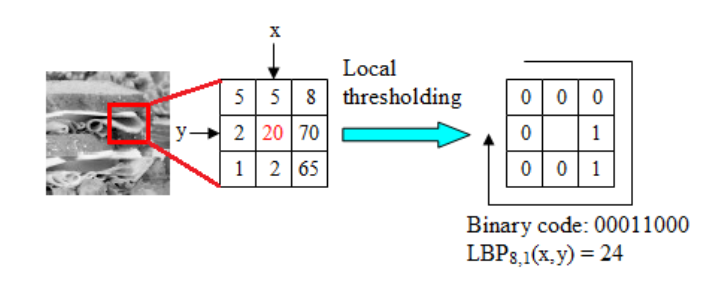
\includegraphics[scale=0.55]{img/lbp}
    \caption{Illustration of the LBP descriptor's process}
    \label{fig:lbp_process}
\end{figure}

Given a pixel $c = (x_c, y_c)$, the value of the $LBP$ code of $c$ is defined as:
$$LBP_{P, R} (x_c, y_c) = \sum_{p = 0}^{P - 1} s (g_p - g_c) 2^p$$
where:
\begin{itemize}
    \item $p$ is a neighbour pixel of $c$ and the distance from $p$ to $c$ does not exceed $R$. Thus, $R$ is the radius of a circle centred in $c$ and $P$ is the numbered of sampled points.
    \item $g_p$ and $g_c$ are the grey values (intensities) of $p$ and $c$
    \item $s(x)$ is the function defined as:
    \begin{equation}
    s(x) =
    \begin{cases}
    1 & \text{if $x \geq 0$}\\
    0 & \text{otherwise} \\
    \end{cases}
    \end{equation}
\end{itemize}

In Fig. \ref{fig:lbp_process}, $R$ and $P$ are 1 and 8 respectively.

The number of histograms bins for $LBP_{P, R}$ is $2^P$.

\subsection{Uniform LBP}

This algorithm has been enhanced to make it rotation invariant. Still in \cite{Ojala2002}, the authors introduce the notion of uniform LBP. A LBP is considered to be uniform if it has at most two bitwise transitions (0 to 1 or 1 to 0 transitions in the binary word). 

For example, the pattern \textit{01000000}  (2 transitions) and \textit{11111110} (1 transition) are both considered to be uniform. For a $LBP_{P, R}$, there is $p + 1$ possible uniforms.

Non-uniform LBP are considered as noise and are assigned the same constant value.

Thus, for uniform LBP, we use the formula:

$$
LBP_{P, R}^{uni} (x_c, y_c) = 
\begin{cases} \displaystyle
\sum_{p = 0}^{P - 1} s (g_p - g_c) 2^p & \text{if uniform} \\
P + 1 & \text{otherwise} \\
\end{cases}
$$

\section{Color descriptor}
\subsection{Color histogram}

HSV space is composed of:
\begin{itemize}
    \item \textbf{Hue} channel: represents the dominant spectral component—colour in its pure form, as in green, red, or yellow
    \item \textbf{Saturation} channel: represents the white added to the pure color (the Hue)
    \item \textbf{Value} channel: represents the brightness of the colour
\end{itemize}

Hue and Saturation corresponds to the chromaticity of the colour. For the joint histogram (2D histogram), the H and S channels are used as value is dependant of the condition where the picture were taken, thus is not interesting. The coordinate system is cylindrical, and is often represented by a six-sided inverted pyramid (see figure \ref{fig:hsv_pyramid}).

\begin{figure}
    \centering
    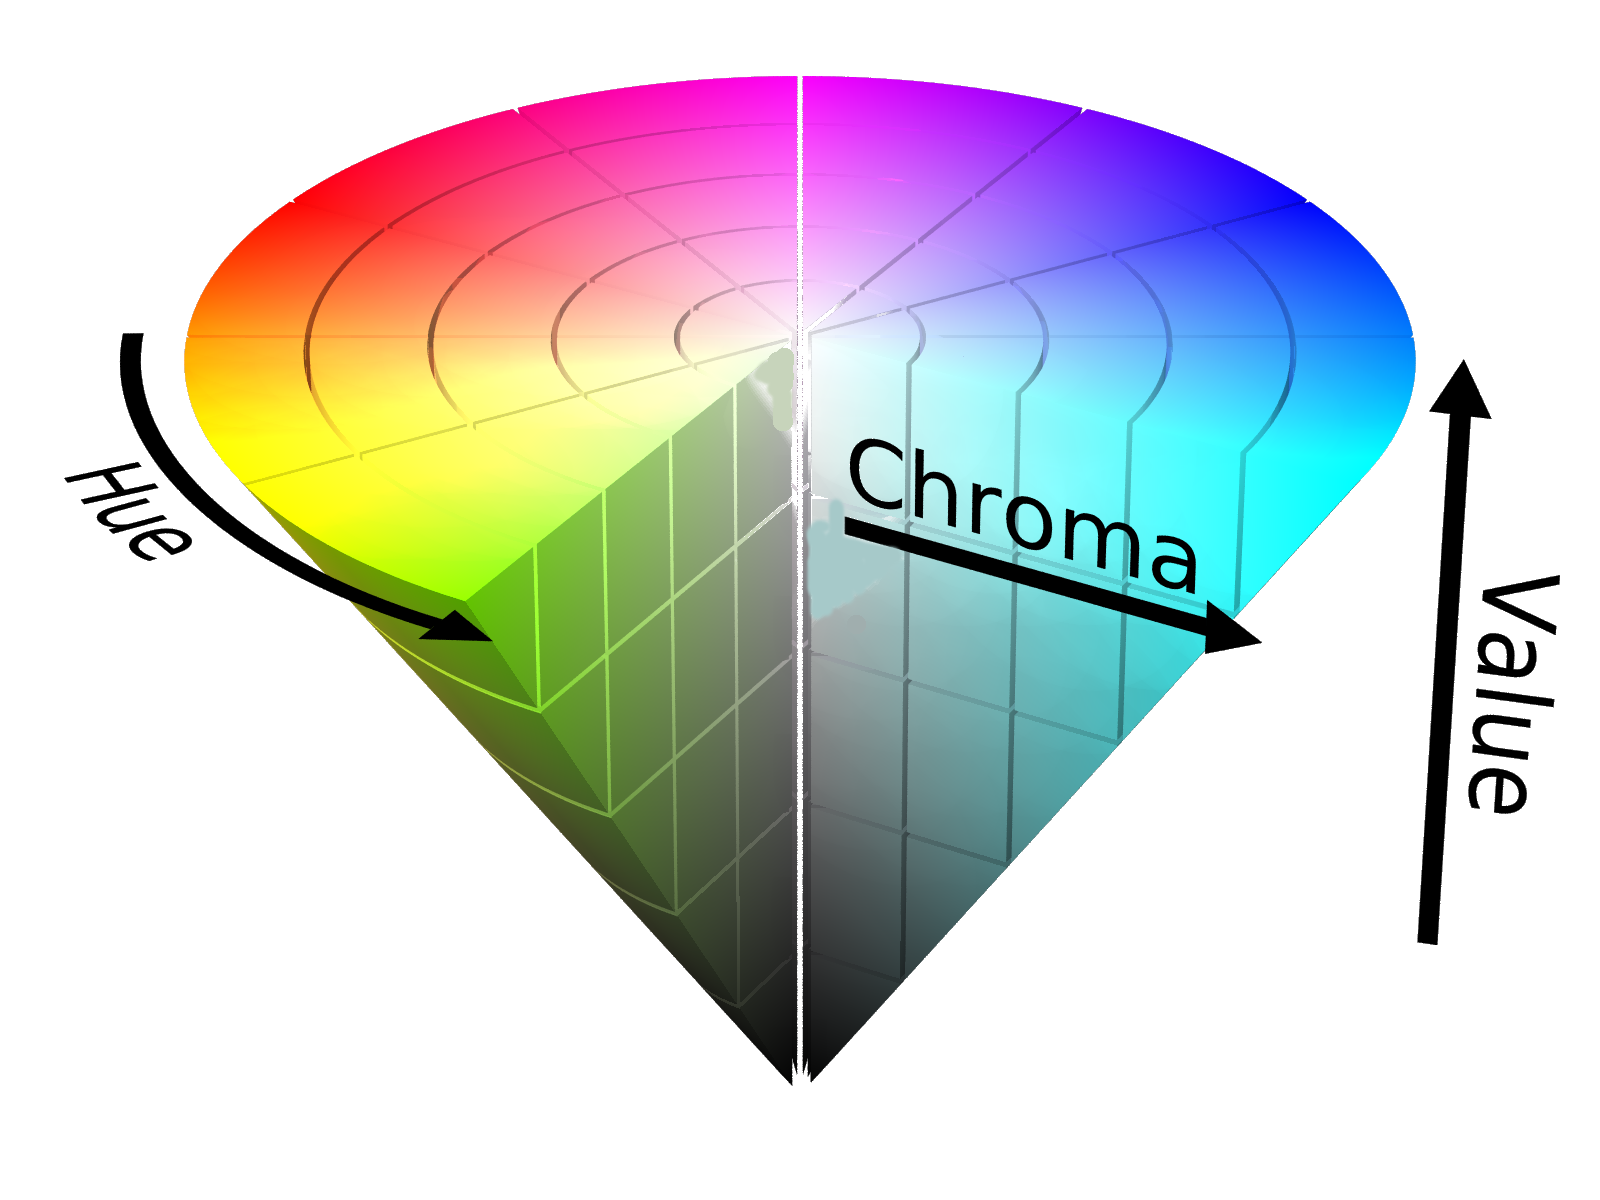
\includegraphics[scale=0.2]{img/HSV_pyramid.png}
    \caption{Pyramid representation of the HSV channels}
    \label{fig:hsv_pyramid}
\end{figure}


\subsection{Color moments}

\subsection{The first two moments}

For a discrete random variable $X$, the first two moments are defined as:
\begin{itemize}
    \item \textbf{Expected value}: $$\E \left[ X \right] = \mu = \sum_{i = 1}^{n} p_i x_i $$
    \item \textbf{Variance}:  $$ \Var (X)= \E \left[ (X - \E \left[ X \right] )^2 \right] =\sum _{i=1}^{n} p_i (x_{i} - \mu )^{2} $$
\end{itemize}

\subsection{Hu moments}

\subsubsection{Raw moments}

For a two-dimensional continuous function f(x,y) the moment (sometimes called \enquote{raw moment}) of (p + q)th order is defined as: 
$$ M_{pq}=\int \limits _{-\infty }^{\infty }\int \limits _{-\infty }^{\infty }x^{p}y^{q}f(x,y) dx dy $$
for $p$ and $q \in \N $.

\subsubsection{Central moments}

And the central moments are :
$$\mu_{pq}=\int \limits_{-\infty }^{\infty }\int \limits _{-\infty}^{\infty} (x- \bar{x})^{p}(y - \bar{y})^{q} f(x,y) dx dy $$
with $\bar{x}=\frac{M_{10}}{M_{00}}$ and $\bar{y}=\frac{M_{01}}{M_{00}}$

\subsubsection{Normalized central moments}

The normalized central moments are:
$$ \eta_{ij}=\frac{\mu _{ij}}{\mu_{00}^{\gamma}} $$
where $\gamma = 1 + \frac{I + j}{2}$ for $i + j \geq 2$.

\subsubsection{Definition of the Hu moments}

On the base of those Moments, Hu in \cite{Hu1962} introduced 7 Moments which are invariant for translation, rotation and resizing:
\begin{align*}
    I_{1} = & \eta _{20}+\eta _{02} \\
    I_{2} = & (\eta _{20}-\eta _{02})^{2}+4\eta _{11}^{2} \\
    I_{3} = & (\eta _{30}-3\eta _{12})^{2}+(3\eta _{21}-\eta _{03})^{2} \\
    I_{4} = & (\eta _{30}+\eta _{12})^{2}+(\eta _{21}+\eta _{03})^{2} \\
    \begin{split}
        I_{5} = & (\eta _{30}-3\eta _{12})(\eta _{30}+\eta _{12})[(\eta _{30}+\eta _{12})^{2}-3(\eta _{21}+\eta _{03})^{2}] \\
        & +(3\eta _{21}-\eta _{03})(\eta _{21}+\eta _{03})[3(\eta _{30}+\eta _{12})^{2} -(\eta _{21}+\eta _{03})^{2}]
    \end{split} \\
    I_{6} = & (\eta _{20}-\eta _{02})[(\eta _{30}+\eta _{12})^{2}-(\eta _{21}+\eta _{03})^{2}]+4\eta _{11}(\eta _{30}+\eta _{12})(\eta _{21}+\eta _{03}) \\
    \begin{split}
        I_{7} = & (3\eta _{21}-\eta _{03})(\eta _{30}+\eta _{12})[(\eta _{30}+\eta _{12})^{2}-3(\eta _{21}+\eta _{03})^{2}] \\
        & - (\eta _{30}-3\eta _{12})(\eta _{21}+\eta _{03})[3(\eta _{30}+\eta _{12})^{2}-(\eta _{21}+\eta _{03})^{2}]
    \end{split} \\
\end{align*}

\section{Bag-of-Words}
\subsection{Process}

\textbf{Bag-of-Words} \textit{BoW}, also called Bag of features, is a feature descriptor method inspired by information retrieval from textual documents.

As illustrated in Fig. \ref{fig:bow_process}, the main steps are:
\begin{itemize}
    \item detecting keypoints on each picture. In my case, I use a dense grid of evenly spaced points at a fixed scale and orientation.
    \item describing each keypoints, i.e. extract a feature vector on a neighbourhood of pixels. SIFT, HOG and SURF are common descriptors.
    \item Generating a fix number of visual words that compose our codebook.
    \item We express each image as an histogram of these words' appearance.
\end{itemize}

The combination of a dense grid and SIFT is commonly called dense SIFT. It has been showed to have greater accuracy than using SIFT for keypoint detection and description.

\begin{figure}
    \centering
    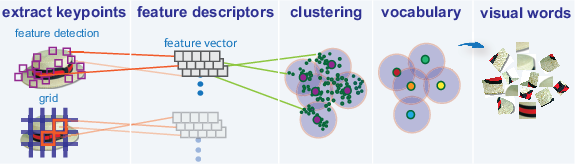
\includegraphics[scale=0.9]{img/bow.png}
    \caption{Illustration of the Bag-Of-Visual-Words model}
    \label{fig:bow_process}
\end{figure}

\subsection{SIFT and SURF}

\textbf{Scale-Invariant Feature Transform} \textit{SIFT} is an algorithm used for detection and description of local feature \cite{Lowe2004}.

The major stages of the algorithm are:
\begin{enumerate}
    \item Scale-space extrema detection: The scale space of an image $L(x, y, \sigma)$ is defined as the product of the convolution of a Gaussian filter $G(x, y, \sigma)$ and an image $I(x, y)$:
    $$
    L(x, y, \sigma) = G(x, y, \sigma) * I(x, y)
    $$
    where $*$ is the convolution at $(x, y)$ and $G(x, y, \sigma) = \frac{1}{2 \pi \sigma^2} \exp(-(x^2 + y^2) / 2 \sigma^2)$.
    
    Laplacian of Gaussian $\sigma^2 \nabla^2 G$ produced the most stable image features but are expensive to compute, thus it is approximated as an Difference of Gaussian (scale-normalized LoG for scale-invariance)
    $$
    G(x, y, k \sigma) - G(x, y, \sigma) \approx (k - 1) \sigma^2 \nabla^2 G
    $$
    
    As presented in figure \ref{fig:sift_difference_of_gaussian}, pyramid of DoG for each octave of scale space is computed: the initial image is repeatedly convolved with Gaussian filters for different values of $\sigma$ to produce the set of scale space images shown on the left. Adjacent Gaussian images are subtracted to produce the difference-of-Gaussian.
    
    \begin{figure}[h]
        \centering
        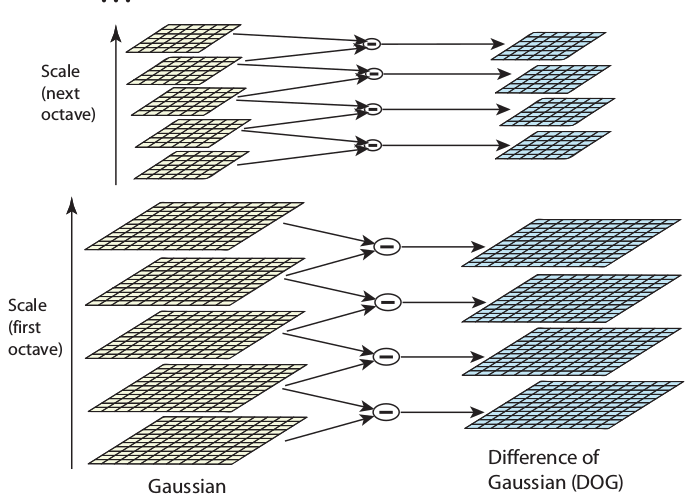
\includegraphics[scale=0.5]{img/sift_difference_of_gaussian.png}
        \caption{Illustration of the difference of Gaussian over multiple octave}
        \label{fig:sift_difference_of_gaussian}
    \end{figure}
    
    \item Keypoint localisation: In order to detect the local maxima and minima of $D(x, y,\sigma)$, each sample point is compared to its eight neighbours in the current image and nine neighbours in the scale above and below. Low contrast and edge keypoints are filtered.
    
    \item Orientation and magnitude assignment: by assigning a consistent orientation to each keypoint based on local image properties, the keypoint descriptor can be represented relative to this orientation and therefore achieve invariance to image rotation.
    
    The magnitude and orientation are defined as:
    $$
    m(x, y) = \sqrt{ \left( L(x +1, y) - L(x -1, y)  \right)^2 + \left( L(x, y + 1) - L(x, y - 1) \right)^2}
    $$
    $$
    \theta(x, y) =\tan^{-1} ( \frac{L(x, y + 1) - L(x, y - 1 )}{L(x + 1, y) - L(x - 1, y)} )
    $$
    
    \item Keypoint descriptor: the local image gradients of a keypoint as presented in figure \ref{fig:sift_descriptor} are computed and accumulated in a histogram. An additional Gaussian weighting function is applied to give less importance to gradients farther away from the keypoint centrer. Once a keypoint candidate has been found by comparing a pixel to its neighbours, the next step is to perform a detailed fit to the nearby data for location, scale, and ratio of principal curvatures. This information allows points to be rejected that have low contrast (and are therefore sensitive to noise) or are poorly localised along an edge.
    
    Usually, SIFT is evaluated at 8 orientation planes over a 4 × 4 neighbourhood giving a
    128-dimension feature vector
    
    \begin{figure}[h]
        \centering
        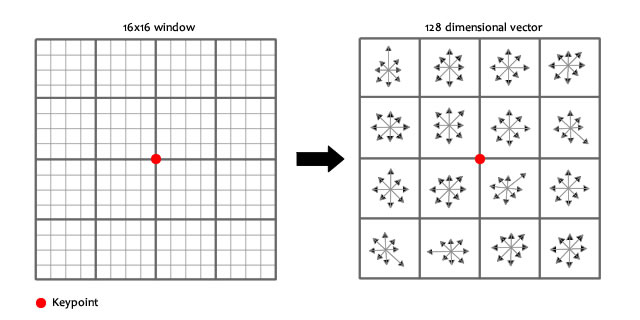
\includegraphics[scale=0.5]{img/sift_descriptor.jpg}
        \caption{Illustration of SIFT as a local image descriptor}
        \label{fig:sift_descriptor}
    \end{figure}
\end{enumerate}

As proven in \cite{Lowe2004}, this method is invariant to translation, scaling and rotation of the picture and is robust to illumination changes, addition of noise, change in the 3-D viewpoint and local geometric distortion.

Multiple variant of SIFT exists. Colour SIFT computes the SIFT in the same manner than the grey scale, except that it does it for each channel independently. Root SIFT is a simple variant of SIFT, presented in \cite{Arandjelovic2012}. When the SIFT descriptors as been computed for each keypoints, we apply an element wise square root of the L1 normalized SIFT vectors


However the SIFT algorithm is quite slow method. That's why in \cite{Bay2006}, the authors present a faster algorithm base on the SIFT approach - \textbf{Speeded Up Robust Features} \textit{SURF}. 
The key is to approximate the LoG with the Box Filter which is the other approximation but of DoG. Using them, the integral image can be constructed and used, which speeds up the whole process since there is no need to iteratively apply those filters one by one (it can be even parallelized). This approach is eagerly applied in the real-time object recognition tasks.

\subsection{K-mean clustering}

Given a set of observations $(x_1, x_2, …, x_n)$, where each observation is a real vector, $k$-means clustering aims to partition the $n$ observations into $k$ $(k \leq n)$ sets $S = {S_1, S_2, …, S_k}$ so as to minimize the within-cluster sum of squares (sum of distance functions of each point in the cluster to its closest centre K). In other words, its objective is to find:

\begin{equation} \label{eq:kmean_objective}
    \underset {S}{\argmin} \sum _{i=1}^{k} \sum _{x \in S_{i}} \left\| x - \mu_{i} \right\|^{2}
\end{equation}

Problem, the exact solution is a NP hard problem. That's why, we can use Lloyd's heuristic algorithm to compute an estimation.

It is an iterative method that find a local minima of the Eq. \ref{eq:kmean_objective}:

\begin{enumerate}
    \item A set of $k$ initial \enquote{means} is chosen randomly within the data domain $M = \{m_1, m_2, \ldots, m_k \}$
    
    \item Then, k clusters are created by associating every observation with the nearest mean.
    $$ \forall i \in \{ 1, \ldots, k \}, ~~ S_{i}^{(t)}= \big \{ x_{p}:{\big \|}x_{p}-m_{i}^{(t)}{\big \|}^{2}\leq {\big \|}x_{p}-m_{j}^{(t)}{\big \|}^{2} ~ \forall j \in \{ 1, \ldots, k \} \big \}$$
    
    \item The centroid of each of the k clusters becomes the new mean.
    $$ \forall i \in \{ 1, \ldots, k \}, ~~ m_{i}^{(t+1)}=\frac {1}{\lvert S_{i}^{(t)} \rvert } \sum _{x_{j} \in S_{i}^{(t)}} x_{j} $$
    
    \item Repeats step 2 and 3 until $M$ not longer changes.
\end{enumerate}

The centroid results and number of iterations are highly dependant of the initial centroid. As a result, the computation is often done several times, with different initialisations.

To help to overcome this issue, the \enquote{kmeans++} initialisation scheme is often used, which has been described in \cite{Arthur2007}. This method initializes the centroids to be (generally) distant from each other, leading to provably better results than random initialization.


\chapter{Classifier}

k-nearest neighborhood

one of the simplest

Tree, random forest

Decision tree: can be used for classification or regression
It can be represented as a graph and a simple representation is given \ref{fig:decision_tree_simple_example}.

\begin{figure}[h]
    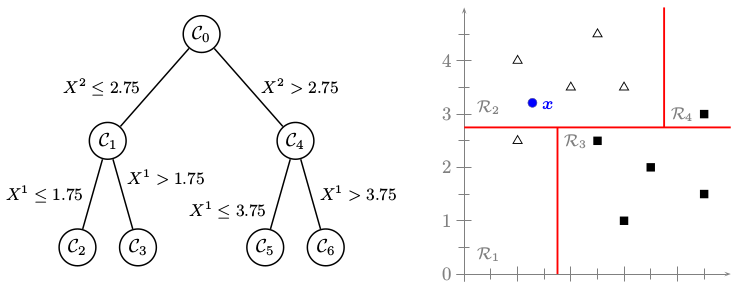
\includegraphics[scale=0.5]{img/decision_tree_simple_example}
    \caption{Decision tree of depth 2 for 10 elements belonging to 2 classes}
    \label{fig:decision_tree_simple_example}
\end{figure}


Naive bayesian

SVM (binary case) + kernel trick + multi-class (one-versus-one or one-versus-all)

The Support Vector Machine (SVM) is a method used for classification and regression. A support vector machine constructs a hyper-plane or set of hyper-planes in a high or infinite dimensional space, which can be used for classification, regression or other tasks. Intuitively, a good separation is achieved by the hyper-plane that has the largest distance to the nearest training data points of any class (so-called functional margin), since in general the larger the margin the lower the generalization error of the classifier.

To generalize SVM to the case of multi-class, multiple approaches are possible:
\begin{itemize}
    \item \enquote{one-versus-one}: train a separate classifier for each different pair of labels. This leads to $\frac{N (N - 1)}{2}$ classifiers
    \item \enquote{one-versus-all}: train a single classifier per class, with the samples of that class as positive samples and all other samples as negatives
\end{itemize}

Kernel trick:
to use the linear SVM for non-linear data: project the data in a new feature H space thanks to an application and then reserch for maximum margin hyperplan in H
to make sure that the new problem has a unique solution, 
must satisfy the Mercer's condition or simply it must be a positiv-definit matrix

\begin{itemize}
    \item \textbf{Linear} : $k(x, y) = \langle \vec{x} , \vec{y} \rangle + C = x^T y + C$
    \item \textbf{Polynomial}: $k(x, y) = (\gamma \cdot \langle \vec{x} , \vec{y} \rangle + C)^d = (\gamma \times x^T y + C)^d$
    \item \textbf{Radial Basis Function (RBF)}: $k(x, y) = \exp \left( - \gamma \lVert x - y \rVert ^2 \right)$
    \item \textbf{Chi-Square}: $\displaystyle k(x, y) = 1 - \sum_{i=1}^n \frac{(x_i-y_i)^2}{\frac{1}{2} (x_i+y_i)}$
    
    A modified version presented in \cite{Vedaldi2010} of this kernel is the \textbf{Additive Chi-Square} kernel :
    $\displaystyle k(x, y) = \sum_{i=1}^n \frac{2 (x_i - y_i)}{x_i + y_i} $
\end{itemize}

The adjustable parameters of these kernels are $d$, $\gamma$, $C$ and must be choosen according to the problem.

SGD classifier + loss function + regularization term% http://scikit-learn.org/stable/modules/sgd.html#mathematical-formulation

CNN

inspired by the neural system composed of different layers and communication shemes
recent years: use of the adjectiv "deep" to qualify NN: many layers

Different types of layers:
% http://cs231n.github.io/convolutional-networks/
% http://caffe.berkeleyvision.org/tutorial/layers.html
% Vision
- convolutional (give the name of the type of NN) : The Convolution layer convolves the input image with a set of learnable filters, each producing one feature map in the output image.
- max pooling
- normalization layer % http://stats.stackexchange.com/a/161200
% Loss layer
- sigmoid
% Activation / Neuron Layers
- ReLu

\chapter{Dataset}  \label{sec:dataset}

Why do we use a dataset?
- learning
- some research make them freely available to test

Describe how it was build ?

\section{Choice of the datatset}

Numerous datasets are already existing and have been made freely available. Creating one's own dataset was an option but it would have been very time consuming and our method's result could not be compared to previous scientific papers.

To choose, a couple of criteria were defined:
\begin{itemize}
    \item Preferably, it should be a recent dataset
    \item It must have a decent number of pictures (a few thousand images)
    \item It must be composed of a general kind of food such as worldwide, Western or Asian
    \item It must contain pictures with multi-food items
\end{itemize}

As we can see in the table \ref{table:dataset_summary}, UEC FOOD 256 is the dataset that best match our expectations.

\begin{table}
    %\setlength{\tabcolsep}{5pt} % Default value: 6pt
    \renewcommand{\arraystretch}{1.1} % Default value: 1
    \begin{tabulary}{\textwidth}{| c | C | C | C | C | C|}
        \hline
        Name & Release date & Number of pictures & Type of food & Number of classes & Multiple food items \\
        \hline
        PFID \cite{Chen2009} & 2009 & 4545 & American fast-food  & 101 & No \\
        \hline
        UEC FOOD 100 \cite{Matsuda2012a} & 2012 & 14361 & Japanese & 100  & Yes \\
        \hline
        FIDS 30 \cite{FIDS30} & 2013 & 971 & Fruit & 30 & No \\
        \hline
        ETHZ Food-101 \cite{Bossard2014} & 2014 & 101 000 & European & 100 & No \\
        \hline
        UPMC Food-101* \cite{Wang2015} & 2015 & 90 840 & European & 100 & No \\
        \hline
        UNICT-FD889 \cite{Farinella2015} & 2015 & 3 583 & World & 889 & No \\
        \hline
        FooDD \cite{ParisaPouladzadehAbdulsalamYassine2015} & 2015 & 3000 & Fruit & 23 & Yes \\
        \hline
        \textbf{UEC FOOD 256} \cite{Kawano2015} & \textbf{2015} & \textbf{31395} & \textbf{World} & \textbf{256}  & \textbf{Yes} \\ 
        \hline
    \end{tabulary}
    \caption[Summary of some available food datasets according to the criteria]{Summary of some available food datasets according to the criteria. \\
        *UPMC FOOD 101 is including the recipe for most of the pictures}
    \label{table:dataset_summary}
\end{table}

\section{UEC FOOD-100 and UEC FOOD-256}

\textbf{UEC FOOD-100} and \textbf{UEC FOOD-256} are datasets used for food localization and recognition.

The UEC FOOD-100 dataset can be found in \footnote{Dataset can be found at \url{http://foodcam.mobi/dataset100.html}}. It was created in 2012 and presented in \cite{Matsuda2012a}.

It contains 100 types of food, mainly Japanese food. Each kind is represented by at least 100 samples.

\begin{figure}[h]
    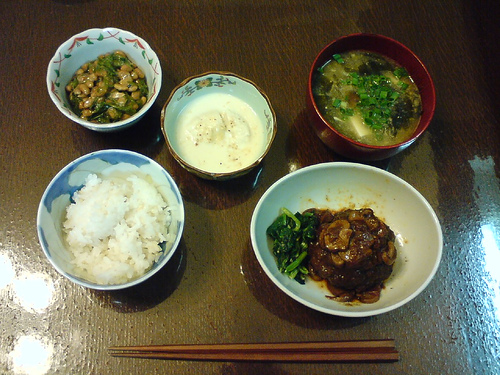
\includegraphics[width=8cm, height=8cm]{img/multiple_food_items_1}
    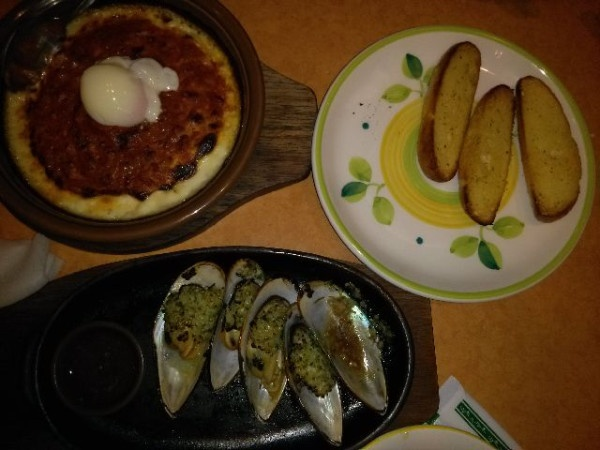
\includegraphics[width=8cm, height=8cm]{img/multiple_food_items_2}
    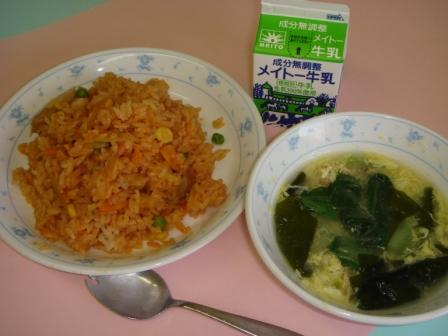
\includegraphics[width=8cm, height=8cm]{img/multiple_food_items_3}
    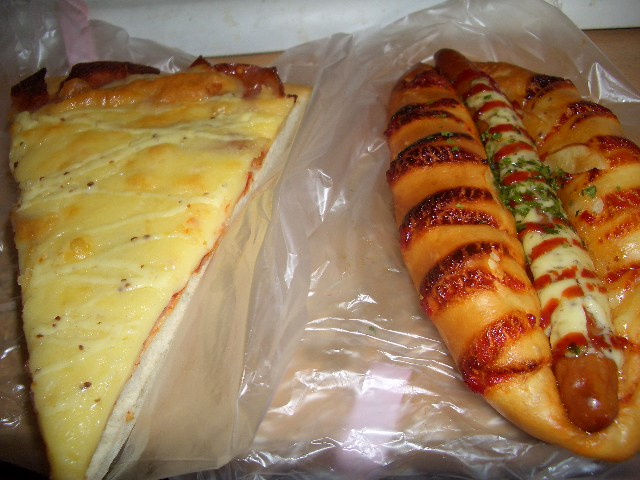
\includegraphics[width=8cm, height=8cm]{img/multiple_food_items_4}
    \caption{Pictures with multiple food items from UEC FOOD 256}
    \label{fig:presentation_multiple_food_items}
\end{figure}

As presented in figure \ref{fig:presentation_multiple_food_items}, a photo can contain more than one food items. The dataset contains files to indicate bounding boxes marking the location of a food items.

UEC FOOD-256 can be found in \footnote{Dataset can be found at \url{http://foodcam.mobi/dataset256.html}}. It was presented in \cite{Kawano2015} in 2015. It contains  the 100 types of food from UEC FOOD-100 plus 156 new ones. The pictures have been automatically  extracted from the Internet and pre-processed. 

The newly introduced food kinds are more international dishes with food from various countries such as France, Italy, the USA, China, Thailand, Vietnam, Japan and Indonesia. As for FOOD 100, every food photo has a bounding box indicating the location of the food item.

The most represented category is miso soup with 728 and rice with 620 pictures.

\chapter{Methodology} \label{sec:methodology}

As illustrated in Fig. \ref{fig:tikz_methodology}, we have our initial dataset that we split in :
\begin{itemize}
    \item a \textbf{validation set} (10 \% of the dataset) used for hyper-parameter optimization or model selection for localisation and classification
    \item a \textbf{train / test set} (remaining dataset) used for the localisation and classification. The train set is used to learn the parameters of a classifier that is then evaluated on the test set (using the same dataset for learning and testing would be a methodological mistake as it would overfit the dataset)
\end{itemize}

\begin{figure}[h]
    \centering
    \tikzstyle{block} = [rectangle, draw, text width=3cm, text centred, rounded corners,  fill=blue!20]
    \tikzstyle{line} = [draw,thick, -latex']
    \tikzstyle{cloud} = [draw, ellipse, text width=3cm, text centred]
    \tikzstyle{edge from parent}=[->,thick,draw]
    \begin{tikzpicture}[auto, edge from parent fork down]
        % Distance between node
        \tikzstyle{level 1}=[sibling distance=80mm,level distance=10ex]
        
        % Place nodes
        \node [cloud, fill=red!10] (base) {Dataset}
        child{node [cloud, fill=green!10] (validation) {Validation set}
            child{node [block, fill=blue!10] (hyperparameter) {Hyper-parameter optimization}}
        }
        child{node [cloud, fill=green!10] (train_test) {Train / test sets}
            child{node [block, fill=blue!10] (localisation) {Localisation}
                child {node[block, fill=blue!10](feature){Feature description}
                    child {node[block, fill=blue!10](classification){Classification}
                        child {node[block, fill=red!10](result){Result}
                        }
                    }
                }
            }
        };
        % Draw edges
        \path [line] (hyperparameter.east) -- (localisation.west);
        \path [line] (hyperparameter.south) -- (classification.west);
    \end{tikzpicture}
    \caption{General process of the localisation and classification}
    \label{fig:tikz_methodology}
\end{figure}

\section{Hyperparameter optimization}

There are numerous parameters that are part of the machine learning but are not learnt. Typical example include which kernel function used (if any) or the value of the penalty parameter $C$ for SVM, the number of $k$ of neighbourhoods for kNN.

We use the exhaustive grid search method to select the parameters that have the highest performance score through 10 fold cross validation. It generates all the possible combination of parameters value and train / test the classifier.

\section{Localisation}

For localisation, a different approach from the literature has been used. The usual way is to detect area of food and non food in a picture. Yet, it was noticed that the food items of UEC FOOD 256 and 100 tends to be in the middle and stands out. Moreover, demanding the user to take pictures that follow these characteristics is reasonable.

That's why a pre-trained CNN used for saliency detection has been used. It has been pre-trained in \cite{zhang2015SOD} on multiple datasets (Multi-Salient-Object, ILSVRC14). It is available \footnote{\url{https://gist.github.com/jimmie33/339fd0a938ed026692267a60b44c0c58}}.

The CNN structure is a copy of \enquote{GoogleNet} model \cite{Szegedy2015}, i.e. it is composed of 22 layers, corresponding to a succession of convolutional, max pooling and activation layers, the last one being a sigmoid function.

The CNN has been pre-trained to detect the likelihood to belong to one of the 100 arbitrary bounding boxes as presented in Fig. \ref{fig:seg_100_bboxes}.

\begin{figure}
    \centering
    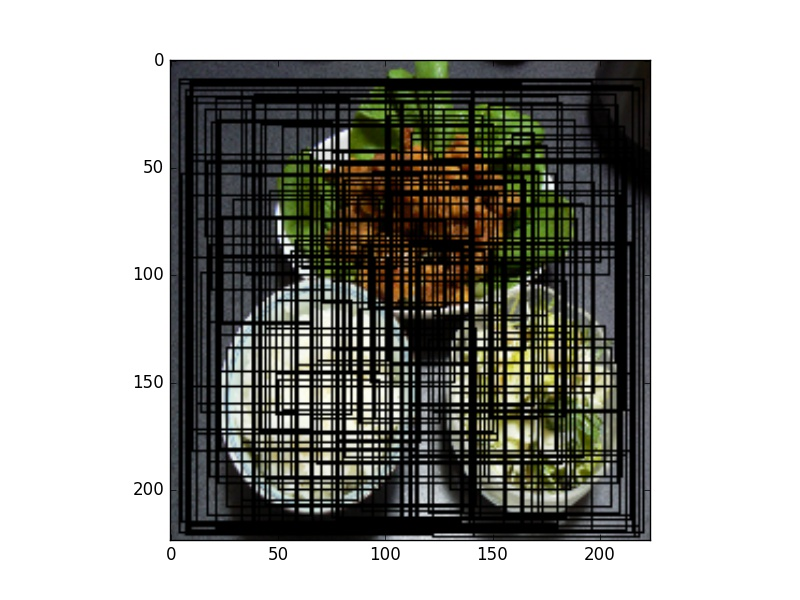
\includegraphics[scale=0.5]{img/seg_100_bboxes.jpg}
    \caption{Picture of the 100 possible bounding boxes that the salient CNN will try to recognise}
    \label{fig:seg_100_bboxes}
\end{figure}

Bounding boxes with a probability higher than a threshold $T$ are selected as candidate (if no box meet this limit, the boundong box with the maximum value is selected). As can be seen in figure \ref{fig:seg_97}, it generates a lot of overlapping copies. That's why, the final step of the localisation process is to discard small bounding boxes and overlapping ones (overlap higher than 30 \%), keeping the ones with highest probabilities.

\begin{figure}
    \centering
    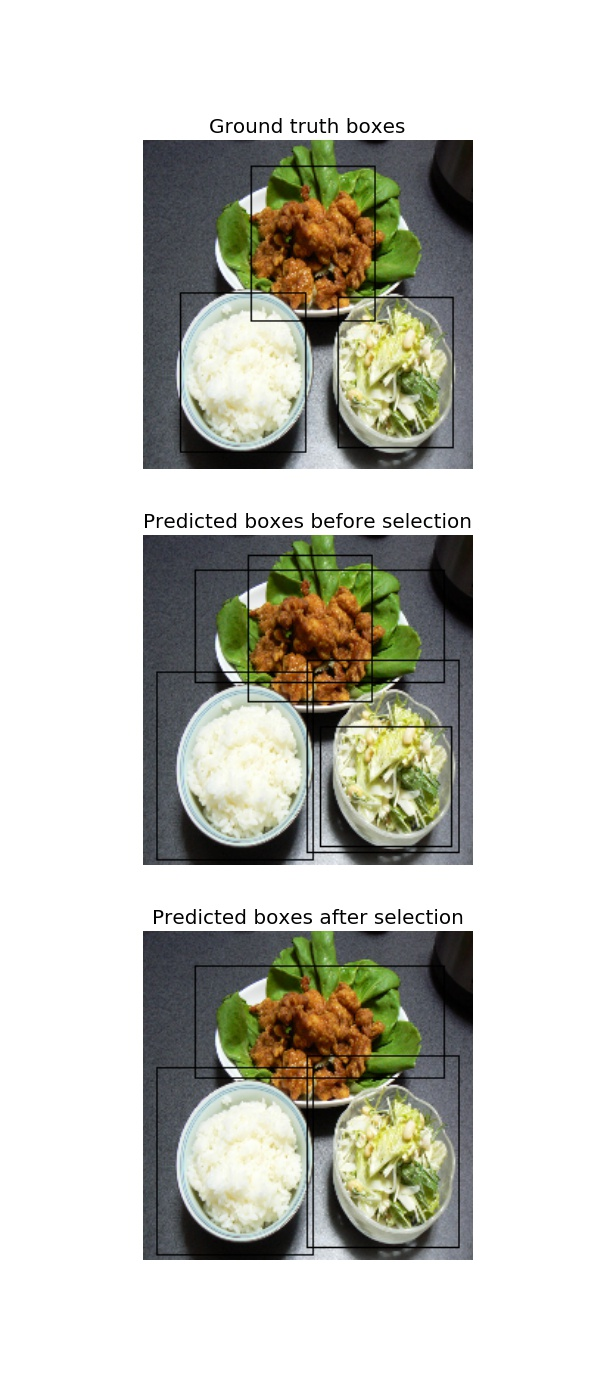
\includegraphics[height=20cm]{img/seg_97.jpg}
    \caption[Segmentation result]{Segmentation process with: the bounding boxes (top), the candidate bounding boxes (middle), the proposed bounding boxes after overlapping suppression (bottom)}
    \label{fig:seg_97}
\end{figure}

\section{Food recognition}
\subsection{Histograms and moments}

The first feature descriptor used combined histograms of LBP with colour moments and histograms for each picture:
\begin{enumerate}
    %\item extract the sub-image delimited by the bounding box
    %\item resize this sub-image to $224 \times 224$ pixels
    \item extract a 100-bin histogram of local binary pattern on the greyscale image
    \item extract a 30-bin by 30-bin joint colour histogram for the channel $H$ and $s$ of the HSV  representation
    \item extract the first two moments of the R, G, B, H, S and Gray channels
    \item extract the 7 Hu moments
\end{enumerate}

The feature vectors are then normalized to have all features centred around zero (mean equal to 0) and have unit variance (equal to 1).

Then, apply multiple classifiers:
\begin{itemize}
    \item decision tree
    \item random forest (made up of 500 trees)
    \item SVM
\end{itemize}

% Talk in result: show the best amelioration with hyperparemeter (but in general it only improve it by one or two percents) ??

\subsection{Bag of words}

\begin{enumerate}
    \item detection of keypoints using a dense grid (4 spaces)
    \item descriptors: Root SIFT. Root SIFT is a simple variant of SIFT, presented in \cite{Arandjelovic2012}. When the SIFT descriptors as been computed for each keypoints, we apply an element wise square root of the L1 normalized SIFT vectors
\end{enumerate}

Then these feature vectors are clustered using the k-means algorithm to obtain a 1000-word codebook.

For each picture, we compute the histogram of occurrence counts of visual words.

This descriptor is used with the SVM classifier and additive $\chi$-squared kernel

\subsection{CNN as a Descriptor}

As described in section \ref{sec:classifier}, a CNN can be used as a feature descriptor. The pre-trained CNN was used for image recognition on ImageNet Challenge 2014 and presented in  \cite{Simonyan2014}. It is available \footnote{\url{https://gist.github.com/ksimonyan/3785162f95cd2d5fee77/}}.

The model is an improved version of the 19-layer model used by the VGG team in the ILSVRC-2014 competition. As the CNN used for segmentation, it takes a $224 \times 224$ RGB picture.

The output of the layer just before the FC is used as a descriptor. Thus, each picture is described by a 4096 feature vectors.

\section{Code}

The code is freely available on Github\footnote{\url{https://github.com/bnogaret/food_log}}.

I'm using python 3.5.2 and its scientific stack bas on Scipy \cite{Oliphant2007}:
\begin{itemize}
    \item Numpy \cite{VanDerWalt2011} for N-dimensional array
    \item Pandas \cite{McKinney2010} for the data structure
    \item Scikit-image \cite{VanderWalt2014} and OpenCV 3 \cite{Bradski2000} for some of the image processing algorithms
    \item Scikit-learn \cite{Pedregosa2012} for most of the machine learning and Caffe \cite{Jia2014a}  for the CNN
    \item Matplotlib \cite{Hunter2007} for 2D graph generation
    \item Sphinx for the documentation
\end{itemize}


\chapter{Evaluation} \label{sec:evaluation}

\section{Environment}

All the code has been run on the \enquote{Astral} high performance computer of Cranfield's university. The operating system is SUSE Linux Enterprise Server 11 (64 bits architecture), with a Linux 3 kernel.

The system is separated in login nodes and compute nodes. There are two \enquote{front-end} login nodes and they contain two Intel E5-2660 (Sandy Bridge - 8 cores) CPUs giving 16 CPU cores and have a total of 192 GB of shared memory. The login nodes enable the user to connect to the system and compile one's program. There are 80 compute nodes, each node having two Intel E5-2660 (Sandy Bridge - 8 cores) CPUs. This is giving a total of 1280 available cores. Each compute node have at least accessed to 64 GB shared memory. Nodes are connected with Infiniband\TM low-latency interconnect.

\section{Segmentation metrics}

To measure the precision of the localisation / segmentation algorithm, we use the metrics as defined in \cite{pascalVoc2012} \footnote{Information on the evaluation system can be found at  \url{http://host.robots.ox.ac.uk/pascal/VOC/voc2012/devkit_doc.pdf}}.

To be considered a correct detection, the \textbf{Intersection over Union} $IoU$ between the predicted bounding box $B_p$ and ground truth bounding box $B_{gt}$ must exceed 50\% by the formula:

$$IoU = \frac{area(B_p \cap B_{gt})}{area(B_p \cup B_{gt})}$$

To simplify the calculation, this formula can be rewritten as:

$$IoU = \frac{area(B_p \cap B_{gt})}{area(B_p) + area(B_{gt}) - area(B_p \cap B_{gt})} $$

Using this metric, we can compute the precision $P$, the recall $R$ and the accuracy $A$ given by:

$$ P =  \frac{T_p}{T_p + F_p}$$
$$ R =  \frac{T_p}{T_p + F_n}$$
$$ A = \frac{T_p}{T_p + F_n + F_p} $$

with:
\begin{itemize}
   \item $T_p$ the number of true positives (the bounding boxes correctly localised)
   \item $F_p$ the number of false positives (the predicted bounding boxes incorrectly localized)
   \item $F_n$ the number of false negative (the ground truth bounding boxes not localized)
\end{itemize}

Note that given the convention from \cite{pascalVoc2012}, if more than one predicted bounding box overlaps the same ground truth bounding box, only one will be considered as $T_P$, the rest will be $F_P$s.

\section{Cross validation}

Cross validation is a technique used to assert the generalization to a new dataset of the different metrics used. 

A common type of cross validation is the k-fold cross validation. In this method, the original sample is randomly split into $k$ partitions of equal sized. Of these generated subsamples, a single split is used for test set, the remaining are used as training data.
This last task is repeated $k$ times, each of the k partitions being used only once for testing. The $k$ results can then be averaged to produce a single estimation (illustrated in figure  \ref{fig:4-fold_cross_validation})

The advantage of this method over repeated random sub-sampling is that all observations are used for both training and testing, each observation being used for testing exactly once. 

10-fold cross-validation were used for all the presented results (the most common fold value that maximises the training set size).

\begin{figure}[h]
    \tikzset{myshade/.style={minimum size=.5cm, outer color ={#1!90!gray}, inner color={#1!90!gray}}}
    \newcommand\myrect[1][]{\tikz\node[rectangle,myshade=#1]{};}
    
    \centering
    \begin{tabular}{rccccl}
        First iteration & \myrect[orange] & \myrect[blue] & \myrect[blue] & \myrect[blue] &\\
        Second iteration & \myrect[blue] & \myrect[orange] & \myrect[blue] & \myrect[blue] & \hspace{1cm} \myrect[blue] : Fold for training \\
        Third iteration & \myrect[blue] & \myrect[blue] & \myrect[orange] & \myrect[blue] & \hspace{1cm} \myrect[orange] : Fold for testing \\
        Fourth iteration & \myrect[blue] & \myrect[blue] & \myrect[blue] & \myrect[orange] &\\
    \end{tabular}
    \caption{Illustration of 4-fold cross validation}
    \label{fig:4-fold_cross_validation}
\end{figure}

\section{Results}

First, the localisation and classification processes were run independently (using the ground truth bounding box for classification).

\subsection{Localisation}

\begin{table}[h]
    \centering
    \renewcommand{\arraystretch}{1.2}
    \begin{tabular}{|c | c c|} 
        \hline
        Metric (average) & My method & DCNN from \cite{Bolanos2016} \\
        \hline
        Accuracy & \textbf{73 \%} & 60 \% \\ 
        \hline
        Recall &  \textbf{74 \%} & 80 \% \\
        \hline
        Precision &  \textbf{79 \%} & 70 \% \\
        \hline
    \end{tabular}
    \caption{Average localisation accuracy result for UEC FOOD 256}
    \label{table:localisation_result}
\end{table}

The table \ref{table:localisation_result} gathers the average accuracy, recall, precision of my localisation method using a DCNN pre-trained on salient object detection. In \cite{Bolanos2016}, the authors use fine-tuned pre-trained Deep Neural Network and obtain around 60 \% of accuracy (using the same IoU over 50 \%).

Compare to the found literature, my method lead to a higher accuracy. It seems that the assumptions made to switch from a DCNN trained to detect food / non-food detection to salient object detection is founded.

For the result of the table \ref{table:localisation_result}, we use an IoU of 50 \%. In Fig \ref{fig:segmentation_overlap}, we can see that the metrics' values are greatly influenced by the threshold choose for correctness (from 73 \% of average accuracy with a threshold at 50 \% to 0 \% of accuracy for a threshold of 100 \%).

\begin{figure}
    \centering
    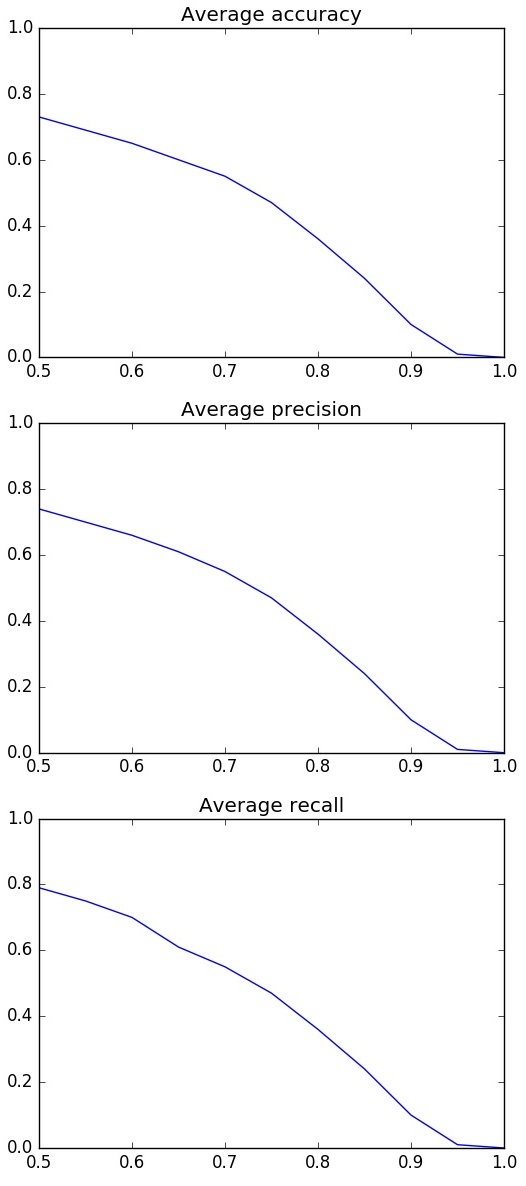
\includegraphics[scale=0.5]{img/segmentation_overlap.jpg}
    \caption{Curves of Accuracy over IoU (top), Precision over IoU (centre) and Recall over IoU (bottom)}
    \label{fig:segmentation_overlap}
\end{figure}

\subsection{Classification}

\begin{table}
    \centering
    \renewcommand{\arraystretch}{1.2}
    \begin{tabulary}{\textwidth}{| c | C|}
        \hline
        Method & Average accuracy \\
        \hline
        CNN as descriptor + RF & \textbf{40 \%} \\ 
        \hline
        BoW (1000 words)+ SVM with $\chi^2$ & 10 \% \\ % made up!
        \hline
        LBP + CHM + Decision tree & 5 \% \\ 
        \hline
        LBP + CHM + SVM & 11 \% \\ % made up!
        \hline
        LBP + CHM + RF & 16 \% \\ % improved!
        \hline
        DCNN from \cite{Bolanos2016} & 63 \%\\
        \hline 
        DCNN from \cite{Yanai2015} & 67 \%\\
        \hline 
    \end{tabulary}
    \caption[Average classification accuracy result for UEC FOOD 256]{Average classification accuracy result for UEC FOOD 256. CHM stands for colour histograms and moments}
\end{table}

In \cite{Bolanos2016}, the authors use a fine-tuned pre-trained Deep Neural Network and obtain 63 \% accuracy on UEC FOOD-256.

In \cite{Yanai2015}, the authors use a fine-tuned pre-trained Deep Neural Network and obtain 67 \% accuracy on UEC FOOD-256.


\subsection{Localisation and classification}

Using the segmentation and classification method with the highest accuracy, i.e. saliency detection DCNN segmenter with DCNN as a feature descriptor and random forest classifier.

The results are presented in the table \ref{table:uecfood100_results}.

\begin{table}
    \centering
    \renewcommand{\arraystretch}{1.2}
    \begin{tabulary}{\textwidth}{| c | C C|}
        \hline
        Process & My method & DCNN from \cite{Bolanos2016} \\
        \hline
        Overall & \textbf{28 \%} & 37 \% \\ 
        \hline
        Localisation &  \textbf{74 \%} & 60 \% \\
        \hline
        Classification &  \textbf{38 \%} & 60 \% \\
        \hline
    \end{tabulary}
    \caption{Average accuracy result for UEC FOOD 256}
    \label{table:uecfodd256_results}
\end{table}

\begin{figure}
    \centering
    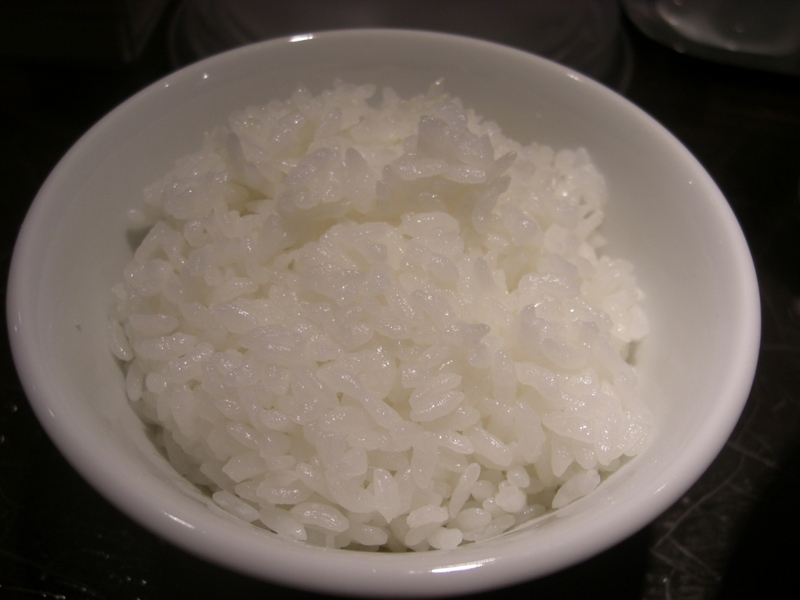
\includegraphics[height=2.5cm, width=2.5cm]{img/top_rice.jpg}
    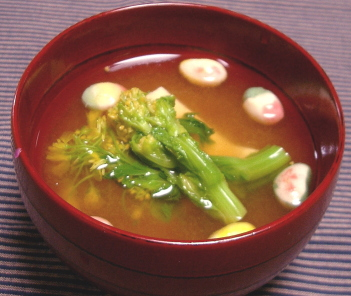
\includegraphics[height=2.5cm, width=2.5cm]{img/top_miso_soup.jpg}
    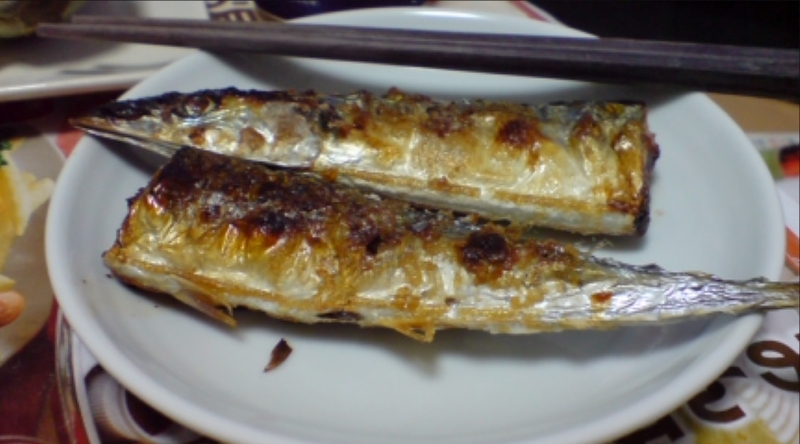
\includegraphics[height=2.5cm, width=2.5cm]{img/top_grilled_pacific_saury.jpg}
    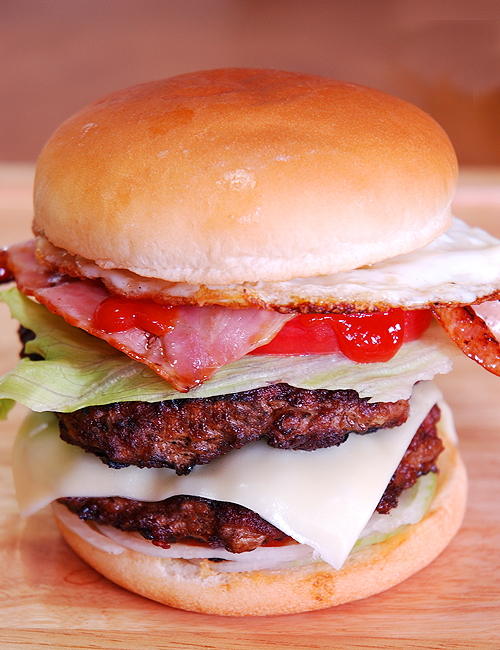
\includegraphics[height=2.5cm, width=2.5cm]{img/top_hamburger.jpg}
    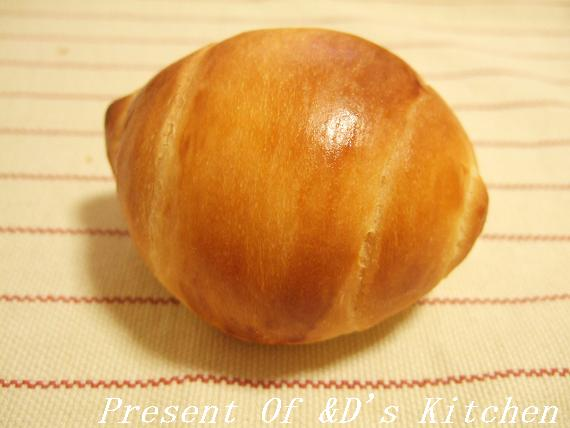
\includegraphics[height=2.5cm, width=2.5cm]{img/top_roll_bread.jpg}
    \caption[Classes having the highest accuracy]{The five classes having the highest accuracy with (from the left to the right, starting from the highest accuracy) rice (98 \%), miso soup (95 \%), grilles pacific saury (94 \%), hamburger (93 \%), roll bread (90 \%)}
    \label{fig:top_5}
\end{figure}

As can been seen in Fig \ref{fig:top_5} and \ref{fig:least_5}, the best performing class is rice and the least one is tanmen. The possible explanations are:
\begin{itemize}
    \item rice is the most represented food items in the dataset, maximising the size of the training sets (same for miso soup)
    \item rice has a specific texture and colour that is relatively invariant to the condition
    \item tanmen is a soup containing noodle and various vegetables. Thus, it can occur in different colour, shape and size.
    \item there are numerous soups in the dataset and tanmen is often confused with them. Figure \ref{fig:confusing_3} show the most class couples that are the most confused and it shows that clear  and miso soup are often mixed up by the method.
\end{itemize}

%14 roll bread 0.905660291919
%17 hamburger 0.936073016618
%49 grilled pacific saury 0.941860410357
%1 rice 0.952117846186
%36 miso soup 0.974164118934

\begin{figure}
    \centering
    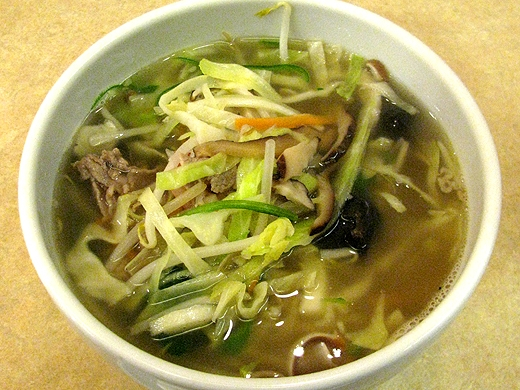
\includegraphics[height=2.5cm, width=2.5cm]{img/least_tanmen.jpg}
    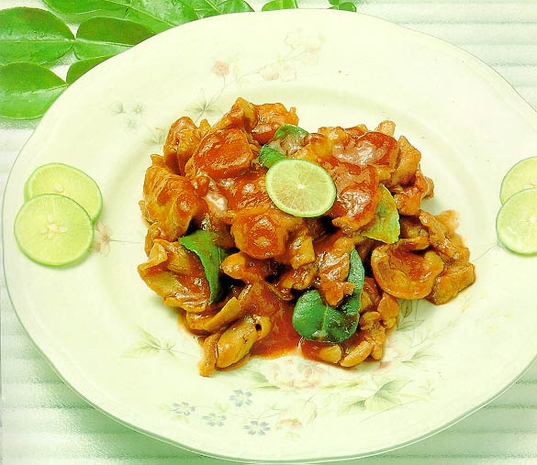
\includegraphics[height=2.5cm, width=2.5cm]{img/least_pork_with_lemon.jpg}
    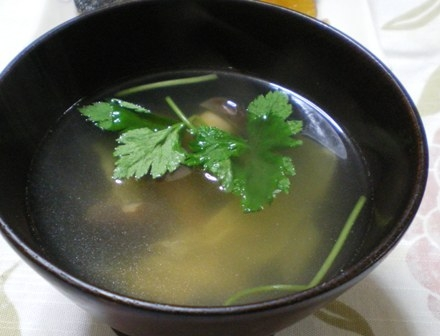
\includegraphics[height=2.5cm, width=2.5cm]{img/least_clear_soup.jpg}
    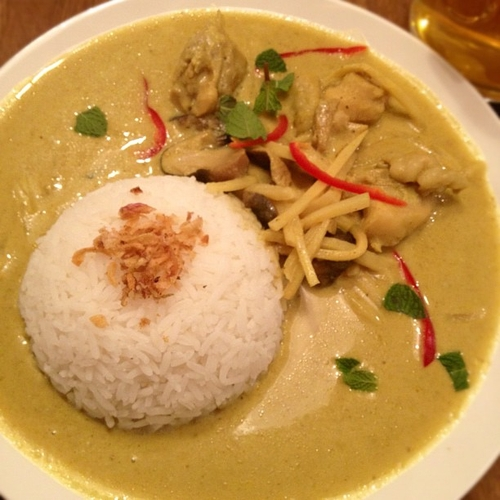
\includegraphics[height=2.5cm, width=2.5cm]{img/least_yellow_curry.jpg}
    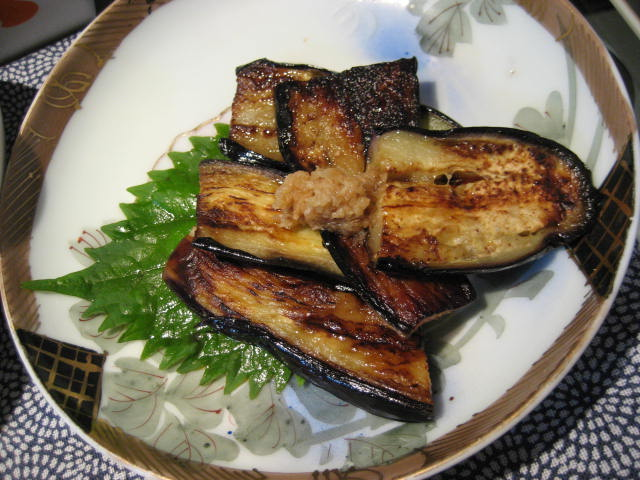
\includegraphics[height=2.5cm, width=2.5cm]{img/least_grilled_eggplant.jpg}
    \caption[Classes having the lowest accuracy]{The five classes having the lowest accuracy with (from the left to the right, starting from the lowest accuracy) tanmen (0 \%), Pork with lemon (0 \%), clear soup (1 \%), yellow curry (1 \%), grilles eggplant (1 \%)}
    \label{fig:least_5}
\end{figure}

%111 tanmen 0.0
%193 Pork with lemon 0.0
%135 clear soup 0.00952380861678
%113 yellow curry 0.0104166655816
%33 grilled eggplant 0.0105263146814

\begin{figure}
    \centering
    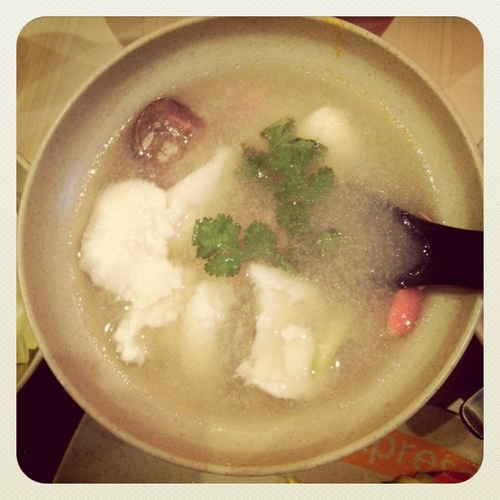
\includegraphics[height=5cm, width=5cm]{img/confusing_clear_soup.jpg}
    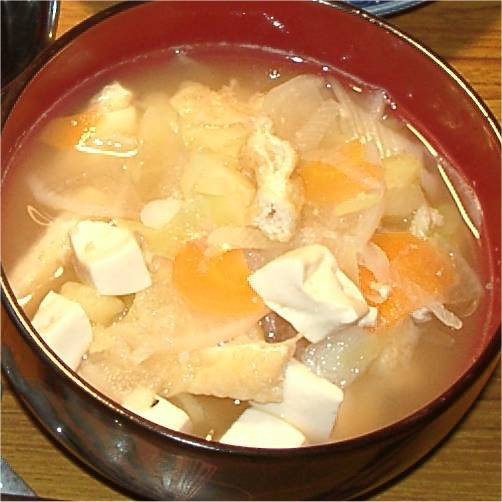
\includegraphics[height=5cm, width=5cm]{img/confusing_miso_soup.jpg}
    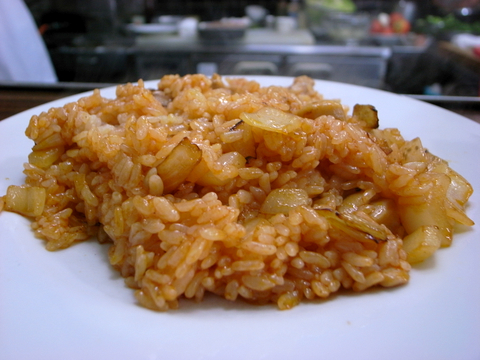
\includegraphics[height=5cm, width=5cm]{img/confusing_chicken_rice.jpg}
    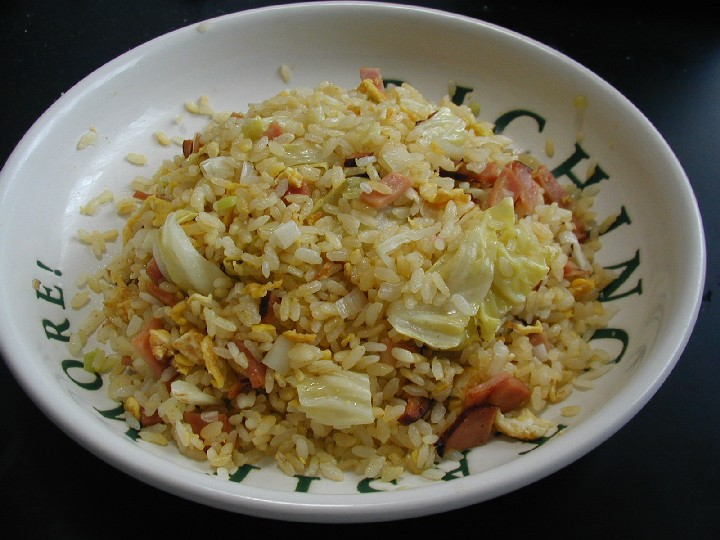
\includegraphics[height=5cm, width=5cm]{img/confusing_fried_rice.jpg}
    \caption[Most confused classes]{The six most confused classes (with from the left to the right, starting from the lowest accuracy) clear soup and miso soup (83 \%), chicken rice and fried rice (54 \%)}
    \label{fig:confusing_3}
\end{figure}

%134 35 clear soup || miso soup 0.838095158277
%88 35 Japanese tofu and vegetable chowder || miso soup 0.754716909932
%124 35 zoni || miso soup 0.727272661157
%156 35 oshiruko or red bean soup || miso soup 0.660194110661
%82 5 cutlet curry || beef curry 0.658914677604
%89 35 pork miso soup || miso soup 0.605504531605
%7 8 chicken rice || fried rice 0.460674105542
%23 22 beef noodle || ramen noodle 0.438596452755
%238 11 kaya toast || toast 0.43434339047
%135 35 yudofu || miso soup 0.431192620992

I also run the segmentation and classification on UEC FOOD 100. The results are presented in table \ref{table:uecfood100_results}. As UEC FOOD 256, it can be seen that the localisation is better than the previous work with 67 \% accuracy (the result is slightly lower than UEC FOOD 256 as it has a higher proportion of multiple food item picture). The overall accuracy is 33 \%.

\begin{table}
    \centering
    \renewcommand{\arraystretch}{1.2}
    \begin{tabulary}{\textwidth}{| C | C c c|} 
        \hline
        Process & My method & DCNN from \cite{Shimoda2015} & DCNN from  \cite{Kawano2014} \\
        \hline
        Overall & \textbf{33 \%} & - & - \\ 
        \hline
        Localisation &  \textbf{67 \%} & 60 \% & - \\
        \hline
        Classification &  \textbf{50 \%} & -  & 72 \% \\
        \hline
    \end{tabulary}
    \caption{Average accuracy result for UEC FOOD 100}
    \label{table:uecfood100_results}
\end{table}


\chapter{Future work} \label{sec:conclusion}

One of the possible future area of work is using a more accurate feature descriptor and / or classifier. Compared to the litterature, my food recognition is rather low. Using a pre-trained DCNN for food recognition seems a promising tool.

It could be also interesting to use multiple segmentation method to combine them.

Then, it can be added the estimation part that include an calorie estimation or a simplified version based on MyPyramid or MyPlate and an application to take picture and visualize user's record.


%% Back matter
%
% This is where we include appendices and references
%
\appendix

\chapter{Appendix}

Structure of the dataset:
a file associating one number ($[1 - 256]$) to a class
a file containing a list of file id containing multiple images
a directory per class: contains the picture. Resolution are all different
	contains a file giving the bounding boxes of this class for each picture
	Thus, we can have the same picture in different directories

\section{RGB to HSV}

Assuming the RGB values have been normalised to be in $[0, 1]$, we have:

\begin{equation*}
    M = \max (R, G, B)
    \qquad
    m = \min (R, G, B)
    \qquad
    C = M - m
\end{equation*}

$$
H =
\begin{cases}
0 & \text{if $C = 0$}\\
60 \times \left[ \frac{G - B}{C} \mod 6\right] & \text{if $M = R$} \\
60 \times \left[ \frac{B - R}{C} + 2\right] & \text{if $M = G$} \\
60 \times \left[ \frac{R - G}{C} + 4\right] & \text{if $M = B$} \\
\end{cases}
$$

$$
S =
\begin{cases}
0 & \text{if $M = 0$}\\
\frac{C}{M}& \text{otherwise} \\
\end{cases}
$$

$$V = M$$

\section{HSV to RGB}

The obtained R, G and B values are in $[0, 1]$ and calculated as such:

\begin{equation*}
    C = V \times S
    \qquad
    X = C \times (1 - \lvert \frac{H}{60} \mod 2 - 1\rvert )
    \qquad
    m = V - C
\end{equation*}

$$
(R', G', B') = 
\begin{cases}
(C, X, 0) & 0 \leq H \leq 60 \\
(X, C, 0) & 60 \leq H \leq 120 \\
(0, C, X) & 120 \leq H \leq 180 \\
(0, X, C) & 180 \leq H \leq 240 \\
(X, 0, C) & 240 \leq H \leq 300 \\
(C, 0, X) & 300 \leq H \leq 360 \\
\end{cases}
$$

$$ (R, G, B) = (R' + m, G' + m, B' + m)$$

% References - you can use BiBTeX inside the 'references' environment if you want.
% For short reference lists, you might find it just as easy to use the bibitem form.
%\begin{references}
%    \bibitem{lamport94}
%        Leslie Lamport,
%        \emph{\LaTeX: a document preparation system}.
%        Addison Wesley, Massachusetts,
%        2nd edition,
%        1994.
%\end{references}
\printbibliography

\end{document}

